%%%%%%%%%%%%%%%%%%%%%%%%%%%%%%%%%%%%%%%%%%%%%%%%%%%%%%%%%%%%%%%%%%%%%%%%%%%%%%%%
% Tutorial slides on Python.
%
% Author: Prabhu Ramachandran <prabhu at aero.iitb.ac.in>
% Copyright (c) 2005-2008, Prabhu Ramachandran
%%%%%%%%%%%%%%%%%%%%%%%%%%%%%%%%%%%%%%%%%%%%%%%%%%%%%%%%%%%%%%%%%%%%%%%%%%%%%%%%

\documentclass[14pt,compress]{beamer}
%\documentclass[draft]{beamer}
%\documentclass[compress,handout]{beamer}
%\usepackage{pgfpages} 
%\pgfpagesuselayout{2 on 1}[a4paper,border shrink=5mm]

% Modified from: generic-ornate-15min-45min.de.tex
\mode<presentation>
{
  \usetheme{Warsaw}
  \useoutertheme{split}
  \setbeamercovered{transparent}
}

\usepackage[english]{babel}
\usepackage[latin1]{inputenc}
%\usepackage{times}
\usepackage[T1]{fontenc}

% Taken from Fernando's slides.
\usepackage{ae,aecompl}
\usepackage{mathpazo,courier,euler}
\usepackage[scaled=.95]{helvet}

\definecolor{darkgreen}{rgb}{0,0.5,0}

\usepackage{listings}
\lstset{language=Python,
    basicstyle=\ttfamily,
    commentstyle=\color{red}\itshape,
  stringstyle=\color{darkgreen},
  showstringspaces=false,
  keywordstyle=\color{blue}\bfseries}

%%%%%%%%%%%%%%%%%%%%%%%%%%%%%%%%%%%%%%%%%%%%%%%%%%%%%%%%%%%%%%%%%%%%%%
% Macros
\setbeamercolor{emphbar}{bg=blue!20, fg=black}
\newcommand{\emphbar}[1]
{\begin{beamercolorbox}[rounded=true]{emphbar} 
      {#1}
 \end{beamercolorbox}
}
\newcounter{time}
\setcounter{time}{0}
\newcommand{\inctime}[1]{\addtocounter{time}{#1}{\tiny \thetime\ m}}

\newcommand{\typ}[1]{\texttt{#1}}

\newcommand{\kwrd}[1]{ \texttt{\textbf{\color{blue}{#1}}}  }

%%% This is from Fernando's setup.
% \usepackage{color}
% \definecolor{orange}{cmyk}{0,0.4,0.8,0.2}
% % Use and configure listings package for nicely formatted code
% \usepackage{listings}
% \lstset{
%    language=Python,
%    basicstyle=\small\ttfamily,
%    commentstyle=\ttfamily\color{blue},
%    stringstyle=\ttfamily\color{orange},
%    showstringspaces=false,
%    breaklines=true,
%    postbreak = \space\dots
% }


%%%%%%%%%%%%%%%%%%%%%%%%%%%%%%%%%%%%%%%%%%%%%%%%%%%%%%%%%%%%%%%%%%%%%%
% Title page
\title[Basic Python]{Python:\\A great programming toolkit}

\author[Asokan \& Prabhu] {Asokan Pichai\\Prabhu Ramachandran}

\institute[IIT Bombay] {Department of Aerospace Engineering\\IIT Bombay}
\date[] {25, July 2009}
%%%%%%%%%%%%%%%%%%%%%%%%%%%%%%%%%%%%%%%%%%%%%%%%%%%%%%%%%%%%%%%%%%%%%%

%\pgfdeclareimage[height=0.75cm]{iitmlogo}{iitmlogo}
%\logo{\pgfuseimage{iitmlogo}}


%% Delete this, if you do not want the table of contents to pop up at
%% the beginning of each subsection:
\AtBeginSubsection[]
{
  \begin{frame}<beamer>
    \frametitle{Outline}
    \tableofcontents[currentsection,currentsubsection]
  \end{frame}
}


% If you wish to uncover everything in a step-wise fashion, uncomment
% the following command: 
%\beamerdefaultoverlayspecification{<+->}

%\includeonlyframes{current,current1,current2,current3,current4,current5,current6}

%%%%%%%%%%%%%%%%%%%%%%%%%%%%%%%%%%%%%%%%%%%%%%%%%%%%%%%%%%%%%%%%%%%%%%
% DOCUMENT STARTS
\begin{document}

\begin{frame}
  \titlepage
\end{frame}
\begin{frame}
  {Acknowledgements}
  \begin{center}
  This program is conducted by\\
  IIT, Bombay\\
  through CDEEP\\as part of  the open source initiatives\\
  under the aegis of\\
  \alert{National Mission on Education through ICT,} \\
  Ministry of HRD.
  \end{center}
\end{frame}

\begin{frame}
  \frametitle{Outline}
  \tableofcontents
  % You might wish to add the option [pausesections]
\end{frame}

%%%%%%%%%%%%%%%%%%%%%%%%%%%%%%%%%%%%%%%%%%%%%%%%%%%%%%%%%%%%%%%%%%%%%%
% TODO
%
%  * Add slide on Python packages (modules)
%  * Add slides on reference counting.

\section{Agenda}
\begin{frame}{About the Workshop}
  \begin{description}
	\item[Session 1] Sat 14:00--15:55
	\item[Session 2] Sat 16:05--18:00
	\item[Session 3] Sun 14:00--15:55
	\item[Session 4] Sun 16:05--18:00 
  \end{description}

  \begin{block}{Goal of the workshop}
	At the end of this program, successful participants will be able to use python as their scripting and problem solving language. Aimed at Engg. students--focus on basic numerics and plotting-- but should serve a similar purpose for others. 
  \end{block}
\end{frame}

\begin{frame}{Checklist}
  Let us verify that all of us are having the same (similar) tools and environment
  \begin{description}
	\item[python] Type python at the command line. Do you see version 2.5 or later?
	\item[IPython] Is IPython available?
	\item[Editor] Which editor? scite, vim, emacs, \ldots
  \end{description}
\end{frame}

\section{Overview}
\begin{frame}{Session 1}
  \begin{itemize}
	\item Introduction and motivation
	\item Using the interpreter(s)
	\item Basic data types: int, float, string
	\item Basic data structures: list
	\item Basic console IO: \texttt{raw\_input(), print}
    \item Basic control flow: \texttt{if, while}
	\item Problem set 1
    \item Functions $\rightarrow$ Problem set 2
    \item lists, \texttt{for}  $\rightarrow$ Problem set 3
    \item IO, Modules $\rightarrow$ Problem sets 4,5, \ldots
  \end{itemize}
\end{frame}

\begin{frame}
  \frametitle{Introduction}
  \begin{itemize}
  \item Creator and BDFL: Guido van Rossum
  \item Conceived in December 1989
  \item ``Python'' as in Monty Python's Flying Circus
  \item Current stable version of Python is 2.6.x
  \item PSF license (like BSD: no strings attached)
  \item Highly cross platform
  \item Runs on the Nokia series 60!
  \item \alert{Philosophy:} Simple and complete by design
  \end{itemize}
\end{frame}

\begin{frame}
  \frametitle{Resources}
  \begin{itemize}
  \item Part of many GNU/Linux distributions
  \item Web: \url{http://www.python.org}
  \item Doc: \url{http://www.python.org/doc}
  \item Free Tutorials:
    \begin{itemize}
    \item Official Python tutorial: \url{http://docs.python.org/tut/tut.html}
    \item Byte of Python: \url{http://www.byteofpython.info/}
    \item Dive into Python: \url{http://diveintopython.org/}
    \end{itemize}
  \end{itemize}
\end{frame}

\begin{frame}
  \frametitle{Why Python?}
  \begin{itemize}
  \item Designed to be readable and easy to use
  \item High level, interpreted, modular, OO
  \item Much faster development cycle
  \item Powerful interactive environment
  \item Rapid application development
  \item Rich standard library and modules
  \item Interfaces well with C++, C and FORTRAN
  \item \alert{More than a math package $\Rightarrow$ some extra work compared to math packages}
  \end{itemize}
\end{frame}

\begin{frame}
  \frametitle{Use cases}
  \begin{itemize}
  \item NASA: Space Shuttle Mission Design
  \item AstraZeneca: Collaborative Drug Discovery
  \item ForecastWatch.com: Helps Meteorologists
  \item Industrial Light \& Magic: Runs on Python
  \item Zope: Commercial grade Toolkit
  \item Plone: Professional high feature CMS
  \item RedHat: install scripts, sys-admin tools
  \item Django: A great web application framework
  \item Google: A strong python shop
  \end{itemize}
\end{frame}

\begin{frame}
  \frametitle{To sum up, python is\ldots}
  \begin{itemize}
  \item dynamically typed, interpreted $\rightarrow$ rapid testing/prototyping
  \item powerful, very high level
  \item has full introspection 
  \item Did we mention powerful?
  \end{itemize}
  \begin{block}{But \ldots}
    may be wanting in performance. specialised resources such as SWIG, \alert{Cython} are available 
  \end{block}
  \inctime{15}
\end{frame}

%%%%%%%%%%%%%%%%%%%%%%%%%%%%%%%%%%%%%%%%%%%%%%%%%%%%%%%%%%%%%%%%%%%%%%
% TIME: 15 m, running 15m
%%%%%%%%%%%%%%%%%%%%%%%%%%%%%%%%%%%%%%%%%%%%%%%%%%%%%%%%%%%%%%%%%%%%%%

\section{Python}

\subsection{Getting Started}

\begin{frame}[fragile]{At the prompt, type the following}
   \begin{lstlisting}
>>> print 'Hello Python' 
>>> print 3124 * 126789
>>> 1786 % 12
>>> 3124 * 126789
>>> a = 3124 * 126789
>>> big = 12345678901234567890 ** 3
>>> verybig = big * big * big * big 
>>> 12345**6, 12345**67, 12345**678
  \end{lstlisting}
\end{frame}

\begin{frame}[fragile]{At the prompt, type the following}
   \begin{lstlisting}
>>> s = 'Hello '
>>> p = 'World'
>>> s + p 
>>> s * 12 
>>> s * s
>>> s + p * 12, (s + p)* 12
>>> s * 12 + p * 12
>>> 12 * s 
    \end{lstlisting}
\end{frame}

\begin{frame}[fragile]{At the prompt, type the following}
  \begin{lstlisting}
>>> 17/2
>>> 17/2.0
>>> 17.0/2
>>> 17.0/8.5
>>> int(17/2.0)
>>> float(17/2)
>>> str(17/2.0)
>>> round( 7.5 )
  \end{lstlisting}
  \begin{block}{Mini exercise}
	Round a float to the nearest integer, using \texttt{int()}?
  \end{block}
\end{frame}

\begin{frame}{Midi exercises}
  \begin{center}
    \begin{itemize}
      \item What does this do?
      \item \texttt{round(amount * 10) /10.0 }
    \end{itemize}
  \end{center}
\end{frame}

\begin{frame}{More exercises?}
  \begin{center}
    \begin{block}{Round sums}
      How to round a number to the nearest  5 paise?\\
      \begin{description}
        \item[Remember] 17.23 $\rightarrow$ 17.25,\\ while 17.22 $\rightarrow$ 17.20\\
      \end{description}
      How to round a number to the nearest 20 paise?
    \end{block}
  \end{center}
\end{frame}

\begin{frame}[fragile] {A question of good style}
  \begin{lstlisting}
    amount = 12.68
    denom = 0.05
    nCoins = round(amount/denom)
    rAmount = nCoins * denom
  \end{lstlisting}
  \pause
  \begin{block}{Style Rule \#1}
    Naming is 80\% of programming
  \end{block}
\end{frame}


\begin{frame}[fragile]
  \frametitle{Odds and ends}
  \begin{itemize}
    \item Case sensitive
    \item Dynamically typed $\Rightarrow$ need not specify a type
      \begin{lstlisting}
a = 1
a = 1.1
a = "Now I am a string!"
      \end{lstlisting}
    \item Comments:
      \begin{lstlisting}
a = 1  # In-line comments
# Comment in a line to itself.
a = "# This is not a comment!"
      \end{lstlisting}
  \end{itemize}
  \inctime{15}
\end{frame}

%%%%%%%%%%%%%%%%%%%%%%%%%%%%%%%%%%%%%%%%%%%%%%%%%%%%%%%%%%%%%%%%%%%%%%
% TIME: 15 m, running 30m
%%%%%%%%%%%%%%%%%%%%%%%%%%%%%%%%%%%%%%%%%%%%%%%%%%%%%%%%%%%%%%%%%%%%%%

\subsection{Data types}
\begin{frame}
  \frametitle{Basic types}
  \begin{itemize}
    \item numbers: float, int, long, complex
    \item strings
    \item boolean
  \end{itemize}
  \begin{block}{Also to be discussed later}
    tuples, lists, dictionaries, functions, objects\ldots
  \end{block}
\end{frame}

\begin{frame}[fragile]
  \frametitle{Numbers}
  \vspace*{-0.25in}
  \begin{lstlisting}
>>> a = 1 # Int.
>>> l = 1000000L # Long
>>> e = 1.01325e5 # float
>>> f = 3.14159 # float
>>> c = 1+1j # Complex!
>>> print f*c/a
(3.14159+3.14159j)
>>> print c.real, c.imag
1.0 1.0
>>> abs(c)
1.4142135623730951
>>> abs( 8 - 9.5 )
1.5
  \end{lstlisting}
\end{frame}

\begin{frame}[fragile]
  \frametitle{Boolean}
  \begin{lstlisting}
>>> t = True
>>> f = not t
False
>>> f or t
True
>>> f and t
False
  \end{lstlisting}
  \begin{block}{Try:}
  NOT True\\
  not TRUE
  \end{block}
\end{frame}

\begin{frame}[fragile]
  \frametitle{Relational and logical operators}
  \begin{lstlisting}
>>> a, b, c = -1, 0, 1
>>> a == b
False
>>> a <= b 
True
>>> a + b != c
True
>>> a < b < c
True
>>> c >= a + b
True
  \end{lstlisting}
\end{frame}

\begin{frame}[fragile]
  \frametitle{Strings}
  \begin{lstlisting}
s = 'this is a string'
s = 'This one has "quotes" inside!'
s = "I have 'single-quotes' inside!"
l = "A string spanning many lines\
one more line\
yet another"
t = """A triple quoted string does
not need to be escaped at the end and 
"can have nested quotes" etc."""
  \end{lstlisting}
\end{frame}

\begin{frame}[fragile]
  \frametitle{More Strings}
  \vspace*{-0.2in}
  \begin{lstlisting}
>>> w = "hello"    
>>> print w[0] + w[2] + w[-1]
hlo
>>> len(w) # guess what
5
>>> s = u'Unicode strings!'
>>> # Raw strings (note the leading 'r')
... r_s = r'A string $\alpha \nu$'
  \end{lstlisting}
\pause
  \begin{lstlisting}
>>> w[0] = 'H' # Can't do that!
Traceback (most recent call last):
  File "<stdin>", line 1, in ?
TypeError: object does not support item assignment
  \end{lstlisting}
\end{frame}

\begin{frame}
  \frametitle{Let us switch to IPython}
  Why?
  \begin{block}
    {Better help (and a lot more)}
    Tab completion\\
    ?\\
    .?\\
    object.function?
  \end{block}
\end{frame}

\begin{frame}[fragile]
  \frametitle{More on strings}
  \begin{lstlisting}
In [1]: a = 'hello world'
In [2]: a.startswith('hell')
Out[2]: True
In [3]: a.endswith('ld')
Out[3]: True
In [4]: a.upper()
Out[4]: 'HELLO WORLD'
In [5]: a.upper().lower()
Out[5]: 'hello world'
  \end{lstlisting}
\end{frame}

\begin{frame}[fragile]{Still with strings}
  \begin{lstlisting}
In [6]: a.split()
Out[6]: ['hello', 'world']
In [7]: ''.join(['a', 'b', 'c'])
Out[7]: 'abc'
In [8] 'd' in ''.join( 'a', 'b', 'c')
Out[8]: False
  \end{lstlisting}
  \begin{block}{Try:}
    \texttt{a.split( 'o' )}\\
    \texttt{'x'.join( a.split( 'o' ) )}
  \end{block}
\end{frame}

\begin{frame}[fragile]{Surprise! strings!!}
  \begin{lstlisting}
In [11]: x, y = 1, 1.2
In [12]: 'x is %s, y is %s' %(x, y)
Out[12]: 'x is 1, y is 1.234'
  \end{lstlisting}
  \begin{block}{Try:}
    \texttt{'x is \%d, y is \%f' \%(x, y) }\\
    \texttt{'x is \%3d, y is \%4.2f' \%(x, y) }
  \end{block}
  \small
\url{docs.python.org/lib/typesseq-strings.html}\\
\end{frame}

\begin{frame}
  {Interlude}
  \begin{block}
    {A classic problem}
    How to interchange values of two variables? Please note that the type of either variable is unknown and it is not necessary that both be of the same type even!
  \end{block}
  \inctime{30}
\end{frame}

%%%%%%%%%%%%%%%%%%%%%%%%%%%%%%%%%%%%%%%%%%%%%%%%%%%%%%%%%%%%%%%%%%%%%%
% TIME: 25 m+ Interlude break 5 mins, running 60m 
%%%%%%%%%%%%%%%%%%%%%%%%%%%%%%%%%%%%%%%%%%%%%%%%%%%%%%%%%%%%%%%%%%%%%%

\subsection{Control flow}
\begin{frame}
  \frametitle{Control flow constructs}  
  \begin{itemize}
  \item \kwrd{if/elif/else}: branching
  \item \kwrd{while}: looping
  \item \kwrd{for}: iterating 
  \item \kwrd{break, continue}: modify loop 
  \item \kwrd{pass}: syntactic filler
  \end{itemize}
\end{frame}

\begin{frame}[fragile]
  \frametitle{Basic conditional flow}
  \begin{lstlisting}
In [21]: a = 7
In [22]: b = 8
In [23]: if a > b:
   ....:    print 'Hello'
   ....: else:
   ....:     print 'World'
   ....:
   ....:
World
  \end{lstlisting}
  Let us switch to creating a file
\end{frame}

\begin{frame}
  {Creating python files}
  \begin{itemize}
    \item aka scripts
    \item use your editor
    \item Note that white space is the way to specify blocks!
    \item extension \typ{.py}
    \item run with \texttt{python hello.py} at the command line
    \item in IPython\ldots
  \end{itemize}
\end{frame}

\begin{frame}[fragile]
  \frametitle{\typ{If...elif...else} example}
\begin{lstlisting}
x = int(raw_input("Enter an integer:"))
if x < 0:
     print 'Be positive!'
elif x == 0:
     print 'Zero'
elif x == 1:
     print 'Single'
else:
     print 'More'
\end{lstlisting}
\end{frame}

\begin{frame}{Simple IO}
  \begin{block}
    {Console Input}
    \texttt{raw\_input(}) waits for user input.\\Prompt string is optional.\\
    All keystrokes are Strings!\\\texttt{int()} converts string to int.
  \end{block}
  \begin{block}
    {Console output}
    \texttt{print} is straight forward. Major point to remember is the distinction between \texttt{print x} and \texttt{print x,}
  \end{block}
\end{frame}

\begin{frame}[fragile]
  \frametitle{Basic looping}
  \begin{lstlisting}
# Fibonacci series:
# the sum of two elements
# defines the next
a, b = 0, 1
while b < 10:
    print b,
    a, b = b, a + b
 
\end{lstlisting}
\typ{1 1 2 3 5 8}\\  
\alert{Recall it is easy to write infinite loops with \kwrd{while}}
  \inctime{20}
\end{frame}

%%%%%%%%%%%%%%%%%%%%%%%%%%%%%%%%%%%%%%%%%%%%%%%%%%%%%%%%%%%%%%%%%%%%%%
% TIME: 20 m, running 80m 
%%%%%%%%%%%%%%%%%%%%%%%%%%%%%%%%%%%%%%%%%%%%%%%%%%%%%%%%%%%%%%%%%%%%%%

\begin{frame}
  \frametitle{Problem set 1}
  \begin{itemize}
    \item All the problems can be\\
      solved using \kwrd{if} and \kwrd{while} 
  \end{itemize}
\end{frame}

\begin{frame}{Problem 1.1}
  Write a program that displays all three digit numbers that are equal to the sum of the cubes of their digits. That is, print numbers $abc$ that have the property $abc = a^3 + b^3 + c^3$\\
These are called $Armstrong$ numbers.
\end{frame}
  
\begin{frame}{Problem 1.2 - Collatz sequence}
\begin{enumerate}
  \item Start with an arbitrary (positive) integer. 
  \item If the number is even, divide by 2; if the number is odd multiply by 3 and add 1.
  \item Repeat the procedure with the new number.
  \item It appears that for all starting values there is a cycle of 4, 2, 1 at which the procedure loops.
\end{enumerate}
    Write a program that accepts the starting value and prints out the Collatz sequence.

\end{frame}

\begin{frame}{Problem 1.3 - Kaprekar's constant}
  \begin{enumerate}
    \item Take a four digit number--with at least two digits different.
    \item Arrange the digits in ascending and descending order, giving A and D respectively.
    \item Leave leading zeros in A!
    \item Subtract A from D.
    \item With the result, repeat from step 2.
  \end{enumerate}
  Write a program to accept a 4-digit number and display the progression to Kaprekar's constant.
\end{frame}

\begin{frame}[fragile]{Problem 1.4}
  Write a program that prints the following pyramid on the screen. 
  \begin{lstlisting}
1
2  2
3  3  3
4  4  4  4
  \end{lstlisting}
The number of lines must be obtained from the user as input.\\
\pause
When can your code fail?
\only<2->{\inctime{25}}
\end{frame}

%%%%%%%%%%%%%%%%%%%%%%%%%%%%%%%%%%%%%%%%%%%%%%%%%%%%%%%%%%%%%%%%%%%%%%
% TIME: 25 m, running 105m 
%%%%%%%%%%%%%%%%%%%%%%%%%%%%%%%%%%%%%%%%%%%%%%%%%%%%%%%%%%%%%%%%%%%%%%

\subsection{Functions}
\begin{frame}[fragile]
\frametitle{Functions: examples}
  \begin{lstlisting}
def signum( r ):
    """returns 0 if r is zero
    -1 if r is negative
    +1 if r is positive"""
    if r < 0:
        return -1
    elif r > 0:
        return 1
    else:
        return 0
  \end{lstlisting}
\end{frame}

\begin{frame}[fragile]
  \frametitle{Functions: examples}
  \begin{lstlisting}
def pad( n, size ): 
    """pads integer n with spaces
    into a string of length size
    """
    SPACE = ' '
    s = str( n )
    padSize = size - len( s )
    return padSize * SPACE + s
  \end{lstlisting}
\pause
What about \%3d?
\end{frame}

\begin{frame}[fragile]
  {What does this function do?}
  \begin{lstlisting}
def what( n ):
    if n < 0: n = -n
    while n > 0:
        if n % 2 == 1:
            return False
        n /= 10
    return True
  \end{lstlisting}
\end{frame}

\begin{frame}[fragile]
  {What does this function do?}
\begin{lstlisting}
def what( n ):
    i = 1    
    while i * i < n:
        i += 1
    return i * i == n, i
  \end{lstlisting}
\end{frame}

\begin{frame}[fragile]
  {What does this function do?}
  \begin{lstlisting}
def what( n, x ):
    z = 1.0
    if n < 0:
        x = 1.0 / x
        n = -n
    while n > 0:
        if n % 2 == 1:
            z *= x
        n /= 2
        x *= x
    return z
  \end{lstlisting}
\end{frame}

\begin{frame}
  {Before writing a function}
  \begin{itemize}
      \item Builtin functions for various and sundry
      \item \typ{abs, any, all, len, max, min}
      \item \typ{pow, range, sum, type}
      \item Refer here:
          \url{http://docs.python.org/library/functions.html}
  \end{itemize}
  \inctime{15} 
\end{frame}
%%%%%%%%%%%%%%%%%%%%%%%%%%%%%%%%%%%%%%%%%%%%%%%%%%%%%%%%%%%%%%%%%%%%%%
% TIME: 15 m, running 120m 
%%%%%%%%%%%%%%%%%%%%%%%%%%%%%%%%%%%%%%%%%%%%%%%%%%%%%%%%%%%%%%%%%%%%%%

\begin{frame}{Problem set 2}
  The focus is on writing functions and calling them.
\end{frame}

\begin{frame}{Problem 2.1}
  Write a function to return the gcd of two numbers.
\end{frame}

\begin{frame}{Problem 2.2}
A pythagorean triad $(a,b,c)$ has the property $a^2 + b^2 = c^2$.\\By primitive we mean triads that do not `depend' on others. For example, (4,3,5) is a variant of (3,4,5) and hence is not primitive. And (10,24,26) is easily derived from (5,12,13) and should not be displayed by our program. \\
Write a program to print primitive pythagorean triads. The program should generate all triads with a, b values in the range 0---100
\end{frame}

\begin{frame}{Problem 2.3}
  Write a program that generates a list of all four digit numbers that have all their digits even and are perfect squares.\\For example, the output should include 6400 but not 8100 (one digit is odd) or 4248 (not a perfect square).
\end{frame}

\begin{frame}{Problem 2.4}
  The aliquot of a number is defined as: the sum of the \emph{proper} divisors of the number. For example, the aliquot(12) = 1 + 2 + 3 + 4 + 6 = 16.\\
  Write a function that returns the aliquot number of a given number. 
\end{frame}

\begin{frame}{Problem 2.5}
  A pair of numbers (a, b) is said to be \alert{amicable} if the aliquot number of a is b and the aliquot number of b is a.\\
  Example: \texttt{220, 284}\\
  Write a program that prints all five digit amicable pairs.
  \inctime{30}
\end{frame}

%%%%%%%%%%%%%%%%%%%%%%%%%%%%%%%%%%%%%%%%%%%%%%%%%%%%%%%%%%%%%%%%%%%%%%
% TIME: 30 m, running 150m 
%%%%%%%%%%%%%%%%%%%%%%%%%%%%%%%%%%%%%%%%%%%%%%%%%%%%%%%%%%%%%%%%%%%%%%

\subsection{Lists}

\begin{frame}[fragile]
  \frametitle{List creation and indexing}
\begin{lstlisting}
>>> a = [] # An empty list.
>>> a = [1, 2, 3, 4] # More useful.
>>> len(a) 
4
>>> a[0] + a[1] + a[2] + a[-1]
10
\end{lstlisting}
  \begin{itemize}
  \item Indices start with ?
  \item Negative indices indicate ?
  \end{itemize}
\end{frame}

\begin{frame}[fragile]
  \frametitle{List: slices}
  \begin{itemize}
  \item Slicing is a basic operation
  \item \typ{list[initial:final:step]}
  \item  The step is optional
  \end{itemize}
\begin{lstlisting}
>>> a[1:3] # A slice.
[2, 3]
>>> a[1:-1]
[2, 3, 4]
>>> a[1:] == a[1:-1]
False  
\end{lstlisting}
Explain last result
\end{frame}

\begin{frame}[fragile]
  \frametitle{List: more slices}
\begin{lstlisting}
>>> a[0:-1:2] # Notice the step!
[1, 3]
>>> a[::2]
[1, 3]
>>> a[-1::-1]
\end{lstlisting}
What do you think the last one will do?
  \emphbar{Note: Strings also use same indexing and slicing.}
\end{frame}

\begin{frame}[fragile]
  \frametitle{List: examples}
\begin{lstlisting}
>>> a = [1, 2, 3, 4]
>>> a[:2]
[1, 3]
>>> a[0:-1:2]
[1, 3]
\end{lstlisting}
\pause
\alert{Lists are mutable (unlike strings)}
\begin{lstlisting}
>>> a[1] = 20
>>> a
[1, 20, 3, 4]
\end{lstlisting}
\end{frame}

\begin{frame}[fragile]
  \frametitle{Lists are mutable and heterogenous}
\begin{lstlisting}
>>> a = ['spam', 'eggs', 100, 1234]
>>> a[2] = a[2] + 23
>>> a
['spam', 'eggs', 123, 1234]
>>> a[0:2] = [1, 12] # Replace items
>>> a
[1, 12, 123, 1234]
>>> a[0:2] = [] # Remove items
>>> a.append( 12345 )
>>> a
[123, 1234, 12345]
\end{lstlisting}
\end{frame}

\begin{frame}[fragile]
  \frametitle{List methods}
\begin{lstlisting}
>>> a = ['spam', 'eggs', 1, 12]
>>> a.reverse() # in situ
>>> a
[12, 1, 'eggs', 'spam']
>>> a.append(['x', 1]) 
>>> a
[12, 1, 'eggs', 'spam', ['x', 1]]
>>> a.extend([1,2]) # Extend the list.
>>> a.remove( 'spam' )
>>> a
[12, 1, 'eggs', ['x', 1], 1, 2]
\end{lstlisting}
\end{frame}

\begin{frame}[fragile]
  \frametitle{List containership}
  \begin{lstlisting}
>>> a = ['cat', 'dog', 'rat', 'croc']
>>> 'dog' in a
True
>>> 'snake' in a
False
>>> 'snake' not in a
True
>>> 'ell' in 'hello world'
True
  \end{lstlisting}
\end{frame}

\begin{frame}[fragile]
  \frametitle{Tuples: immutable}
\begin{lstlisting}
>>> t = (0, 1, 2)
>>> print t[0], t[1], t[2], t[-1] 
0 1 2 2
>>> t[0] = 1
Traceback (most recent call last):
  File "<stdin>", line 1, in ?
TypeError: object does not support item
           assignment
\end{lstlisting}  
\begin{itemize}
    \item Multiple return values are actually a tuple.
    \item Exchange is tuple (un)packing
\end{itemize}

\end{frame}

\begin{frame}[fragile]
  \frametitle{\typ{range()} function}
  \begin{lstlisting}
>>> range(7)
[0, 1, 2, 3, 4, 5, 6]
>>> range( 3, 9)
[3, 4, 5, 6, 7, 8]
>>> range( 4, 17, 3)
[4, 7, 10, 13, 16]
>>> range( 5, 1, -1)
[5, 4, 3, 2]
>>> range( 8, 12, -1)
[]
  \end{lstlisting}
\end{frame}

\begin{frame}[fragile]
  \frametitle{\typ{for\ldots range(\ldots)} idiom}
  \begin{lstlisting}
In [83]: for i in range(5):
   ....:     print i, i * i
   ....:     
   ....:     
0 0
1 1
2 4
3 9
4 16
\end{lstlisting}
\end{frame}

\begin{frame}[fragile]
  \frametitle{\typ{for}: the list companion}
  
  \begin{lstlisting}
In [84]: a = ['a', 'b', 'c']
In [85]: for x in a:
   ....:    print x, chr( ord(x) + 10 )
   ....:
a  k
b  l
c  m
  \end{lstlisting}
  Iterating over the list and not the index + reference\\
  what if you want the index?
\end{frame}

\begin{frame}[fragile]
  \frametitle{\typ{for}: the list companion}
  \begin{lstlisting}
In [89]: for p, ch in enumerate( a ):
   ....:     print p, ch
   ....:     
   ....:     
0 a
1 b
2 c
  \end{lstlisting}
Try: \typ{print enumerate(a)}
\inctime{20}
\end{frame}

%%%%%%%%%%%%%%%%%%%%%%%%%%%%%%%%%%%%%%%%%%%%%%%%%%%%%%%%%%%%%%%%%%%%%%
% TIME: 20 m, running 170m 
%%%%%%%%%%%%%%%%%%%%%%%%%%%%%%%%%%%%%%%%%%%%%%%%%%%%%%%%%%%%%%%%%%%%%%

\begin{frame}
  {Problem set 3}
  As you can guess, idea is to use \kwrd{for}!
\end{frame}

\begin{frame}{Problem 3.1}
  Which of the earlier problems is simpler when we use \kwrd{for} instead of \kwrd{while}? 
\end{frame}

\begin{frame}{Problem 3.2}
  Given an empty chessboard and one Bishop placed in any square, say (r, c), generate the list of all squares the Bishop could move to.
\end{frame}

\begin{frame}[fragile]
  \frametitle{Problem 3.3}

  Given two real numbers \typ{a, b}, and an integer \typ{N}, write a
  function named \typ{linspace( a, b, N)} that returns an ordered list
  of \typ{N} points starting with \typ{a} and ending in \typ{b} and
  equally spaced.\\

  For example, \typ{linspace(0, 5, 11)}, should return, \\
\begin{lstlisting}
[ 0.0 ,  0.5,  1.0 ,  1.5,  2.0 ,  2.5,  
  3.0 ,  3.5,  4.0 ,  4.5,  5.0 ]
\end{lstlisting}
\end{frame}

\begin{frame}[fragile]
  \frametitle{Problem 3.4a (optional)}

Use the \typ{linspace} function and generate a list of N tuples of the form\\
\typ{[($x_1$,f($x_1$)),($x_2$,f($x_2$)),\ldots,($x_N$,f($x_N$))]}\\for the following functions,\begin{itemize}
  \item \typ{f(x) = sin(x)}
  \item \typ{f(x) = sin(x) + sin(10*x)}.
\end{itemize}
\end{frame}

\begin{frame}[fragile]
  \frametitle{Problem 3.4b (optional)}

  Using the tuples generated earlier, determine the intervals where the roots of the functions lie.

  \inctime{15}
\end{frame}

%%%%%%%%%%%%%%%%%%%%%%%%%%%%%%%%%%%%%%%%%%%%%%%%%%%%%%%%%%%%%%%%%%%%%%
% TIME: 15 m, running 185m 
%%%%%%%%%%%%%%%%%%%%%%%%%%%%%%%%%%%%%%%%%%%%%%%%%%%%%%%%%%%%%%%%%%%%%%

\subsection{IO}

\begin{frame}[fragile]
  \frametitle{Simple tokenizing and parsing}
  \begin{lstlisting}
s = """The quick brown fox jumped
       over the lazy dog"""
for word in s.split():
    print word.capitalize()
  \end{lstlisting}
\end{frame}

\begin{frame}[fragile]
  \frametitle{Problem 4.1}
  Given a string like, ``1, 3-7, 12, 15, 18-21'', produce the list \\
  \begin{lstlisting}
    [1,3,4,5,6,7,12,15,18,19,20,21]
  \end{lstlisting}
\end{frame}

\begin{frame}[fragile]
  \frametitle{File handling}
\begin{lstlisting}
>>> f = open('/path/to/file_name')
>>> data = f.read() # Read entire file.
>>> line = f.readline() # Read one line.
>>> f.close() # close the file.
\end{lstlisting}
Writing files
\begin{lstlisting}
>>> f = open('/path/to/file_name', 'w')
>>> f.write('hello world\n')
>>> f.close()
\end{lstlisting}
\begin{itemize}
    \item Everything read or written is a string
\end{itemize}
\emphbar{Try \typ{file?} for more help}
\end{frame}

\begin{frame}[fragile]
    \frametitle{File and \kwrd{for}}
\begin{lstlisting}
>>> f = open('/path/to/file_name')
>>> for line in f:
...     print line
...
\end{lstlisting}
\end{frame}

\begin{frame}{Problem 4.2}
    The given file has lakhs of records in the form:\\
    \typ{RGN;ID;NAME;MARK1;\ldots;MARK5;TOTAL;PFW}\\
    Some entries may be empty.  Read the data from this file and print the
    name of the student with the maximum total marks.
\end{frame}

\begin{frame}{Problem 4.3}
    For the same data file compute the average marks in different
    subjects, the student with the maximum mark in each subject and also
    the standard deviation of the marks.  Do this efficiently.

    \inctime{20}
\end{frame}

%%%%%%%%%%%%%%%%%%%%%%%%%%%%%%%%%%%%%%%%%%%%%%%%%%%%%%%%%%%%%%%%%%%%%%
% TIME: 20 m, running 205m 
%%%%%%%%%%%%%%%%%%%%%%%%%%%%%%%%%%%%%%%%%%%%%%%%%%%%%%%%%%%%%%%%%%%%%%

\subsection{Modules}

\begin{frame}[fragile]
    {Modules}
\begin{lstlisting}
>>> sqrt(2)
Traceback (most recent call last):
  File "<stdin>", line 1, in <module>
NameError: name 'sqrt' is not defined
>>> import math        
>>> math.sqrt(2)
1.4142135623730951
\end{lstlisting}
\end{frame}

\begin{frame}[fragile]
    {Modules}
  \begin{itemize}
    \item The \kwrd{import} keyword ``loads'' a module
    \item One can also use:
      \begin{lstlisting}
>>> from math import sqrt
>>> from math import *
      \end{lstlisting}    
    \item What is the difference?
    \item \alert{Use the later only in interactive mode}
    \end{itemize}
  \emphbar{Package hierarchies}
      \begin{lstlisting}
>>> from os.path import exists
      \end{lstlisting}
\end{frame}

\begin{frame}
  \frametitle{Modules: Standard library}
  \begin{itemize}
  \item Very powerful, ``Batteries included''
  \item Some standard modules:
    \begin{itemize}
    \item Math: \typ{math}, \typ{random}
    \item Internet access: \typ{urllib2}, \typ{smtplib}
    \item System, Command line arguments: \typ{sys}
    \item Operating system interface: \typ{os}
    \item Regular expressions: \typ{re}
    \item Compression: \typ{gzip}, \typ{zipfile}, and \typ{tarfile}
    \item And a whole lot more!
    \end{itemize}
  \item Check out the Python Library reference:
    \url{http://docs.python.org/library/}
  \end{itemize}
\end{frame}

\begin{frame}[fragile]
    {Modules of special interest}
    \begin{description}[matplotlibfor2d]

        \item[\typ{numpy}] Efficient, powerful numeric arrays

        \item[\typ{matplotlib}] Easy, interactive, 2D plotting

        \item[\typ{scipy}] statistics, optimization, integration, linear
            algebra, Fourier transforms, signal and image processing,
            genetic algorithms, ODE solvers, special functions, and more

        \item[Mayavi] Easy, interactive, 3D plotting

    \end{description}
\end{frame}

\begin{frame}[fragile]
    {Creating your own modules}
  \begin{itemize}
  \item Define variables, functions and classes in a file with a
    \typ{.py} extension
  \item This file becomes a module!
  \item Accessible when in the current directory
  \item Use \typ{cd} in IPython to change directory

  \item Naming your module
      \end{itemize}
\end{frame}

\begin{frame}[fragile]
  \frametitle{Modules: example}
  \begin{lstlisting}
# --- arith.py ---
def gcd(a, b):
    if a%b == 0: return b
    return gcd(b, a%b)
def lcm(a, b):
    return a*b/gcd(a, b)
# ------------------
>>> import arith
>>> arith.gcd(26, 65)
13
>>> arith.lcm(26, 65)
130
  \end{lstlisting}
\end{frame}

\begin{frame}[fragile]
  \frametitle{Problem 5.1}

  Put all the functions you have written so far as part of the problems
  into one module called \typ{iitb.py} and use this module from IPython.

\inctime{20}
\end{frame}
%%%%%%%%%%%%%%%%%%%%%%%%%%%%%%%%%%%%%%%%%%%%%%%%%%%%%%%%%%%%%%%%%%%%%%
% TIME: 20 m, running 225m 
%%%%%%%%%%%%%%%%%%%%%%%%%%%%%%%%%%%%%%%%%%%%%%%%%%%%%%%%%%%%%%%%%%%%%%

\begin{frame}
  \frametitle{Did we meet the goal?}
  \tableofcontents
  % You might wish to add the option [pausesections]
  \end{frame}

  \begin{frame}
    {Tomorrow}
    \begin{itemize}
      \item Plotting: 2D, 3D
      \item NumPy, SciPy
      \item Dictionary, Set
      \item Debugging
      \item Testing
      \item \ldots
    \end{itemize}
    11:30--13:00 Discussion of answers to problems OPTIONAL
  \end{frame}
\end{document}


\begin{frame}[fragile]
  \frametitle{More on functions}
  \begin{itemize}
  \item Support default and keyword arguments
  \item Scope of variables in the function is local
  \item Mutable items are \alert{passed by reference}
  \item First line after definition may be a documentation string
    (\alert{recommended!})
  \item Function definition and execution defines a name bound to the
    function
  \item You \emph{can} assign a variable to a function!
  \end{itemize}
\end{frame}


\begin{frame}[fragile]
  \frametitle{Functions: default arguments}
  \begin{lstlisting}
def ask_ok(prompt, retries=4, complaint='Yes or no!'):
    while True:
        ok = raw_input(prompt)
        if ok in ('y', 'ye', 'yes'): 
            return True
        if ok in ('n', 'no', 'nop', 'nope'): 
            return False
        retries = retries - 1
        if retries < 0: 
            raise IOError, 'bad user'
        print complaint
  \end{lstlisting}
\end{frame}

\begin{frame}[fragile]
  \frametitle{Functions: keyword arguments}
  \begin{lstlisting}
def parrot(voltage, state='a stiff', 
           action='voom', type='Norwegian Blue'):
    print "-- This parrot wouldn't", action,
    print "if you put", voltage, "Volts through it."
    print "-- Lovely plumage, the", type
    print "-- It's", state, "!"

parrot(1000)
parrot(action = 'VOOOOOM', voltage = 1000000)
parrot('a thousand', state = 'pushing up the daisies')
parrot('a million', 'bereft of life', 'jump')
\end{lstlisting}
\end{frame}

\begin{frame}[fragile]
  \frametitle{Functions: arbitrary argument lists}
  \begin{itemize}
  \item Arbitrary number of arguments using \verb+*args+ or
    \verb+*whatever+
  \item Keyword arguments using \verb+**kw+
  \item Given a tuple/dict how do you call a function?
    \begin{itemize}
    \item Using argument unpacking
    \item For positional arguments: \verb+foo(*[5, 10])+
    \item For keyword args: \verb+foo(**{'a':5, 'b':10})+
    \end{itemize}
  \end{itemize}
\begin{lstlisting}
def foo(a=10, b=100):
    print a, b
def func(*args, **keyword):
    print args, keyword
# Unpacking:
args = [5, 10]
foo(*args)
kw = {'a':5, 'b':10}
foo(**kw)
\end{lstlisting}
\end{frame}

\subsection{Modules, exceptions, classes}

\begin{frame}
  \frametitle{Modules}
  \begin{itemize}
  \item Define variables, functions and classes in a file with a
    \typ{.py} extension
  \item This file becomes a module!
  \item Modules are searched in the following:
    \begin{itemize}
    \item Current directory
    \item Standard: \typ{/usr/lib/python2.3/site-packages/} etc.
    \item Directories specified in PYTHONPATH
    \item \typ{sys.path}: current path settings (from the \typ{sys}
      module)
    \end{itemize}
  \item The \typ{import} keyword ``loads'' a module
  \item One can also use:
    \mbox{\typ{from module import name1, name2, name2}}\\
    where \typ{name1} etc. are names in the module, ``module''
  \item \typ{from module import *} \ --- imports everything from module,
    \alert{use only in interactive mode}
  \end{itemize}
\end{frame}

\begin{frame}[fragile]
  \frametitle{Modules: example}
  \begin{lstlisting}
# --- foo.py ---
some_var = 1
def fib(n): # write Fibonacci series up to n
    """Print a Fibonacci series up to n."""
    a, b = 0, 1
    while b < n:
        print b,
        a, b = b, a+b
# EOF

>>> import foo
>>> foo.fib(10)
1 1 2 3 5 8 
>>> foo.some_var
1
  \end{lstlisting}
\end{frame}

\begin{frame}[fragile]
  \frametitle{Namespaces}
  \begin{itemize}
  \item A mapping from names to objects
  \item Modules introduce a namespace 
  \item So do classes
  \item The running script's namespace is \verb+__main__+
  \item A modules namespace is identified by its name
  \item The standard functions (like \typ{len}) are in the
    \verb+__builtin__+ namespace
  \item Namespaces help organize different names and their bindings to
    different objects
  \end{itemize}
\end{frame}

\begin{frame}
  \frametitle{Exceptions}
  \begin{itemize}
  \item Python's way of notifying you of errors
  \item Several standard exceptions: \typ{SyntaxError}, \typ{IOError}
    etc.
  \item Users can also \typ{raise} errors
  \item Users can create their own exceptions
  \item Exceptions can be ``caught'' via \typ{try/except} blocks
  \end{itemize}
\end{frame}

\begin{frame}[fragile]
  \frametitle{Exception: examples}
\begin{lstlisting}
>>> 10 * (1/0)
Traceback (most recent call last):
  File "<stdin>", line 1, in ?
ZeroDivisionError: integer division or modulo by zero
>>> 4 + spam*3
Traceback (most recent call last):
  File "<stdin>", line 1, in ?
NameError: name 'spam' is not defined
>>> '2' + 2
Traceback (most recent call last):
  File "<stdin>", line 1, in ?
TypeError: cannot concatenate 'str' and 'int' objects
\end{lstlisting}
\end{frame}

\begin{frame}[fragile]
  \frametitle{Exception: examples}
\begin{lstlisting}
>>> while True:
...     try:
...         x = int(raw_input("Enter a number: "))
...         break
...     except ValueError:
...         print "Invalid number, try again..."
...
>>> # To raise exceptions
... raise ValueError, "your error message"
Traceback (most recent call last):
  File "<stdin>", line 2, in ?
ValueError: your error message
\end{lstlisting}
\end{frame}

\begin{frame}[fragile]
  \frametitle{Classes: the big picture}
  \begin{itemize}
  \item Lets you create new data types
  \item Class is a template for an object belonging to that class
  \item Note: in Python a class is also an object
  \item Instantiating a class creates an instance (an object)
  \item An instance encapsulates the state (data) and behavior
    (methods)
  \item Allows you to define an inheritance hierarchy
    \begin{itemize}
    \item ``A Honda car \alert{is a} car.''
    \item ``A car \alert{is an} automobile.''
    \item ``A Python \alert{is a} reptile.''
    \end{itemize}
  \item Programmers need to think OO
  \end{itemize}
\end{frame}

\begin{frame}[fragile]
  \frametitle{Classes: what's the big deal?}
  \begin{itemize}
  \item Lets you create objects that mimic a real problem being
    simulated
  \item Makes problem solving more natural and elegant
  \item Easier to create code
  \item Allows for code-reuse
  \item Polymorphism
  \end{itemize}
\end{frame}

\begin{frame}[fragile]
  \frametitle{Class definition and instantiation}
  \begin{itemize}
  \item Class definitions when executed create class objects
  \item Instantiating the class object creates an instance of the
    class
  \end{itemize}
\footnotesize
\begin{lstlisting}
class Foo(object):
    pass
# class object created.
# Create an instance of Foo.
f = Foo()
# Can assign an attribute to the instance
f.a = 100
print f.a
100
\end{lstlisting}
\end{frame}

\begin{frame}[fragile]
  \frametitle{Classes \ldots}
  \begin{itemize}
  \item All attributes are accessed via the \typ{object.attribute}
    syntax
  \item Both class and instance attributes are supported
  \item \emph{Methods} represent the behavior of an object: crudely
    think of them as functions ``belonging'' to the object
  \item All methods in Python are ``virtual''
  \item Inheritance through subclassing
  \item Multiple inheritance is supported
  \item No special public and private attributes: only good
    conventions
    \begin{itemize}
    \item \verb+object.public()+: public
    \item \verb+object._private()+ \& \verb+object.__priv()+: 
      non-public
    \end{itemize}
  \end{itemize}
\end{frame}

\begin{frame}[fragile]
  \frametitle{Classes: examples}
\begin{lstlisting}
class MyClass(object):
    """Example class (this is the class docstring)."""
    i = 12345 # A class attribute
    def f(self):
        """This is the method docstring"""
        return 'hello world'

>>> a = MyClass() # creates an instance
>>> a.f()
'hello world'
>>> # a.f() is equivalent to MyClass.f(a)
... # This also explains why f has a 'self' argument.
... MyClass.f(a)
'hello world'
\end{lstlisting}
\end{frame}

\begin{frame}[fragile]
  \frametitle{Classes (continued)}
  \begin{itemize}
  \item \typ{self} is \alert{conventionally} the first argument for a
    method
  \item In previous example, \typ{a.f} is a method object
  \item When \typ{a.f} is called, it is passed the instance \typ{a} as
    the first argument
  \item If a method called \verb+__init__+ exists, it is called when
    the object is created
  \item If a method called \verb+__del__+ exists, it is called before
    the object is garbage collected
  \item Instance attributes are set by simply ``setting'' them in
    \typ{self}
  \item Other special methods (by convention) like \verb+__add__+ let
    you define numeric types:
    {\footnotesize \url{http://docs.python.org/ref/specialnames.html}
      \\ \url{http://docs.python.org/ref/numeric-types.html}
    }
  \end{itemize}
\end{frame}

\begin{frame}[fragile]
  \frametitle{Classes: examples}
\begin{lstlisting}
class Bag(MyClass): # Shows how to derive classes
    def __init__(self): # called on object creation.
        self.data = [] # an instance attribute
    def add(self, x):
        self.data.append(x)
    def addtwice(self, x):
        self.add(x)
        self.add(x)
>>> a = Bag()
>>> a.f() # Inherited method
'hello world'
>>> a.add(1); a.addtwice(2)
>>> a.data
[1, 2, 2]
\end{lstlisting}
\end{frame}

\begin{frame}[fragile]
  \frametitle{Derived classes}
  \begin{itemize}
  \item Call the parent's \verb+__init__+ if needed
  \item If you don't need a new constructor, no need to define it in subclass
  \item Can also use the \verb+super+ built-in function
  \end{itemize}
\begin{lstlisting}
class AnotherBag(Bag):
    def __init__(self):
        # Must call parent's __init__ explicitly
        Bag.__init__(self)
        # Alternatively use this:
        super(AnotherBag, self).__init__()
        # Now setup any more data.
        self.more_data = []
\end{lstlisting}
\end{frame}

\begin{frame}[fragile]
  \frametitle{Classes: polymorphism}
\begin{lstlisting}
class Drawable(object):
    def draw(self):
        # Just a specification.
        pass
\end{lstlisting}
\mode<presentation>{\pause}
\begin{lstlisting}
class Square(Drawable):
    def draw(self):
        # draw a square.
class Circle(Drawable):
    def draw(self):
        # draw a circle.
\end{lstlisting}
\mode<presentation>{\pause}
\begin{lstlisting}
class Artist(Drawable):
    def draw(self):
        for obj in self.drawables:
            obj.draw()
\end{lstlisting}
\end{frame}

\subsection{Miscellaneous}

\begin{frame}[fragile]
  \frametitle{Stand-alone scripts}
Consider a file \typ{f.py}:
\begin{lstlisting}
#!/usr/bin/env python
"""Module level documentation."""
# First line tells the shell that it should use Python
# to interpret the code in the file.
def f():
    print "f"

# Check if we are running standalone or as module.
# When imported, __name__ will not be '__main__'
if __name__ == '__main__':
    # This is not executed when f.py is imported.
    f() 
\end{lstlisting}
\end{frame}

\begin{frame}[fragile]
  \frametitle{List comprehensions}
\begin{lstlisting}
>>> veg = ['tomato', 'cabbage', 'carrot', 'potato']
>>> [x.upper() for x in veg]
['TOMATO', 'CABBAGE', 'CARROT', 'POTATO']
>>> vec = range(0, 8)
>>> even = [x for x in vec if x%2 == 0]
>>> even
[0, 2, 4, 6]
>>> [x*x for x in even]
[0, 4, 16, 36]
>>> odd = [x for x in vec if x%2 == 1]
>>> odd
[1, 3, 5, 7]
>>> [x*y for x in even for y in odd]
[0, 0, 0, 0, 2, 6, 10, 14, 4, 12, 20, 28, 6, 18,30,42]
\end{lstlisting}
\end{frame}

\begin{frame}[fragile]
  \frametitle{More IPython features}
  \begin{itemize}
  \item Input and output caching:
    \begin{itemize}
    \item \verb+In+: a list of all entered input
    \item \verb+Out+: a dict of all output
    \item \verb+_+, \verb+__+, \verb+__+ are the last three results as
      is \verb+_N+
    \item \verb+%hist [-n]+ macro shows previous history, \verb+-n+
      suppresses line number information
    \end{itemize}
  \item Log the session using \verb+%logstart+, \verb+%logon+ and
    \verb+%logoff+
  \item \verb+%run [options] file[.py]+ -- running Python code
    \begin{itemize}
    \item \verb+%run -d [-b<N>]+: debug script with pdb
          \verb+N+ is the line number to break at (defaults to 1)
    \item \verb+%run -t+: time the script
    \item \verb+%run -p+: Profile the script
    \end{itemize}
  \item \verb+%prun+ runs a statement/expression under the profiler
  \item \verb+%macro [options] macro_name n1-n2 n3-n4 n6+ save specified
    lines to a macro with name \verb+macro_name+
  \end{itemize}
\end{frame}

\begin{frame}[fragile]
  \frametitle{More IPython features \ldots}
  \begin{itemize}
  \item \verb+%edit [options] [args]+: edit lines of code or file
    specified in editor (configure editor via \verb+$EDITOR+)
  \item \verb+%cd+ changes directory, see also \verb+%pushd, %popd, %dhist+
  \item Shell access
    \begin{itemize}
    \item \verb+!command+ runs a shell command and returns its output
    \item \verb+files = %sx ls+ or \verb+files = !ls+ sets
      \verb+files+ to all result of the \verb+ls+ command
    \item \verb+%sx+ is quiet
    \item \verb+!ls $files+ passes the \verb+files+ variable to the
      shell command
    \item \verb+%alias alias_name cmd+ creates an alias for a system
      command
    \end{itemize}
  \item \verb+%colors+ lets you change the color scheme to
    \verb+NoColor, Linux, LightBG+
  \end{itemize}
\end{frame}

\begin{frame}[fragile]
  \frametitle{More IPython features \ldots}
  \begin{itemize}
  \item Use \verb+;+ at the end of a statement to suppress printing
    output
  \item \verb+%bookmark+: store a bookmarked location, for use with \verb+%cd+
  \item \verb+%who, %whos+: print information on variables
  \item \verb+%save [options] filename n1-n2 n3-n4+: save lines to a
    file
  \item \verb+%time statement+: Time execution of a Python statement or
    expression
  \item \verb+%timeit [-n<N> -r<R> [-t|-c]] statement+: time execution
    using Python's timeit module
  \item Can define and use profiles to setup IPython differently:
    \verb+math, scipy, numeric, pysh+ etc.
  \item \verb+%magic+: \alert{Show help on all magics}
  \end{itemize}
\end{frame}

\begin{frame}[fragile]
  \frametitle{File handling}
\begin{lstlisting}
>>> # Reading files:
... f = open('/path/to/file_name')
>>> data = f.read() # Read entire file.
>>> line = f.readline() # Read one line.
>>> # Read entire file appending each line into a list
... lines = f.readlines()
>>> f.close() # close the file.
>>> # Writing files:
... f = open('/path/to/file_name', 'w')
>>> f.write('hello world\n')
\end{lstlisting}
  \begin{itemize}
  \item \typ{tell()}: returns int of current position
  \item \typ{seek(pos)}: moves current position to specified byte
  \item Call \typ{close()} when done using a file
  \end{itemize}
\end{frame}

\begin{frame}[fragile]
  \frametitle{Math}
  \begin{itemize}
  \item \typ{math} module provides basic math routines for
    floats
  \item \typ{cmath} module provides math routies for complex
    numbers
  \item \typ{random}: provides pseudo-random number generators
    for various distributions
  \item These are always available and part of the standard library
  \item More serious math is provided by the NumPy/SciPy modules --
    these are not standard and need to be installed separately
  \end{itemize}
\end{frame}

\begin{frame}[fragile]
  \frametitle{Timing and profiling}
  \begin{itemize}
  \item Timing code: use the \typ{time} module
  \item Read up on \typ{time.time()} and \typ{time.clock()}
  \item \typ{timeit}: is a better way of doing timing
  \item IPython has handy \typ{time} and \typ{timeit} macros (type
    \typ{timeit?} for help)
  \item IPython lets you debug and profile code via the \typ{run}
    macro (type \typ{run?} on the prompt to learn more)
  \end{itemize}
\end{frame}

\begin{frame}[fragile]
  \frametitle{Odds and ends}
  \begin{itemize}
  \item \typ{dir([object])} function: attributes of given object
  \item \typ{type(object)}: returns type information
  \item \typ{str(), repr()}: convert object to string representation
  \item \typ{isinstance, issubclass}
  \item \typ{assert} statements let you do debugging assertions in
    code
  \item \typ{csv} module: reading and writing CSV files
  \item \typ{pickle}: lets you save and load Python objects
    (\alert{serialization})
  \item \typ{sys.argv}: command line arguments
  \item \typ{os.path}: common path manipulations
  \item Check out the Python Library reference:
    \url{http://docs.python.org/lib/lib.html}
  \end{itemize}
\end{frame}

\begin{frame}[fragile]
  \frametitle{Test driven development (TDD)}
  \begin{itemize}
      \item Why?
          \begin{itemize}

            \item Forces you to write reusable code!

            \item Think about the API

            \item More robust

            \item Makes refactoring very easy

          \end{itemize}
      \item How?  Python offers three major ways of doing this
          \begin{itemize}
              \item doctest
              \item unittest
              \item nosetest (and similar like py.test)
          \end{itemize}

      \item Test every piece of functionality you offer

      \item This isn't a formal introduction but more a practical one

  \end{itemize}
\end{frame}

\begin{frame}[fragile]
  \frametitle{Unit test}
\begin{lstlisting}
import unittest

class MyTestCase(unittest.TestCase):
    def setUp(self):
        # Called *before* each test_* 
    def tearDown(self):
        # Called *after* each test_* 
    def test_something(self):
        "docstring"
        #  Test code.
        self.assertEqual(x, y)
        self.assertRaises(ValueError, func, arg1, arg2 ...)

if __name__ == '__main__':
    unittest.main() 
\end{lstlisting}
\end{frame}

\begin{frame}[fragile]
    \frametitle{Nosetest}
\begin{lstlisting}
import particle
def test_particle():
    # Use asserts here.
    p = particle.Particle(1.0)
    assert p.property[0] == 1.0
    assert p.property[2] == 0.0

if __name__ == '__main__':
    import nose
    nose.main()
\end{lstlisting}
\end{frame}

\begin{frame}[fragile]
  \frametitle{Testing}
  \begin{itemize}
      \item More details: see library reference and search for nosetest
  \end{itemize}
\end{frame}

\section{Numerics \& Plotting}

\subsection{NumPy Arrays}

\newcommand{\num}{\texttt{numpy}}

\begin{frame}
  \frametitle{The \num\ module}
  \begin{itemize}
  \item Manipulating large Python lists for scientific computing is
    \alert{slow}
  \item Most complex computations can be reduced to a few standard
    operations
  \item The \num\ module provides:
    \begin{itemize}
    \item An efficient and powerful array type for various common data
      types
    \item Abstracts out the most commonly used standard operations on
      arrays
    \end{itemize}
  \item Numeric was the first, then came \texttt{numarray}.
    \texttt{numpy} is the latest and is the future
  \item This course uses \num\ and only covers the absolute basics
  \end{itemize}
\end{frame}

\begin{frame}
  \frametitle{Basic concepts}
  \begin{itemize}
  \item \num\ arrays are of a fixed size (\typ{arr.size}) and have the
    same type (\typ{arr.dtype})
  \item \num\ arrays may have arbitrary dimensionality
  \item The \typ{shape} of an array is the extent (length) of the
    array along each dimension
  \item The \typ{rank(arr)} of an array is the ``dimensionality'' of the
    array
  \item The \typ{arr.itemsize} is the number of bytes (8-bits) used for
    each element of the array
  \item \alert{Note:} The \typ{shape} and \typ{rank} may change as
    long as the \typ{size} of the array is fixed
  \item \alert{Note:} \typ{len(arr) != arr.size} in general
  \item \alert{Note:} By default array operations are performed
    \alert{elementwise}
  \item Indices start from 0
  \end{itemize}
\end{frame}

\begin{frame}[fragile]
  \frametitle{Examples of \num}
\begin{lstlisting}
# Simple array math example
>>> from numpy import *
>>> a = array([1,2,3,4])
>>> b = array([2,3,4,5])
>>> a + b # Element wise addition!
array([3, 5, 7, 9])

>>> print pi, e  # Pi and e are defined.
3.14159265359 2.71828182846
# Create array from 0 to 10
>>> x = arange(0.0, 10.0, 0.05)
>>> x *= 2*pi/10 # multiply array by scalar value
array([ 0.,0.0314,...,6.252])
# apply functions to array.
>>> y = sin(x)
\end{lstlisting}
\end{frame}

\begin{frame}[fragile]
  \frametitle{More examples of \num}
\vspace*{-8pt}
\begin{lstlisting}
# Size, shape, rank, type etc.
>>> x = array([1., 2, 3, 4])
>>> size(x)
4
>>> x.dtype # or x.dtype.char
'd'
>>> x.shape
(4,)
>>> print rank(x), x.itemsize
1 8
>>> x.tolist()
[1.0, 2.0, 3.0, 4.0]
# Array indexing
>>> x[0] = 10
>>> print x[0], x[-1]
10.0 4.0
\end{lstlisting}
\end{frame}

\begin{frame}[fragile]
  \frametitle{Multi-dimensional arrays}
\begin{lstlisting}
>>> a = array([[ 0, 1, 2, 3],
...            [10,11,12,13]])
>>> a.shape # (rows, columns)
(2, 4)
# Accessing and setting values
>>> a[1,3] 
13
>>> a[1,3] = -1
>>> a[1] # The second row
array([10,11,12,-1])

# Flatten/ravel arrays to 1D arrays
>>> a.flat  # or ravel(a)
array([0,1,2,3,10,11,12,-1])
# Note: flat references original memory
\end{lstlisting}
\end{frame}

\begin{frame}[fragile]
  \frametitle{Slicing arrays}
\begin{lstlisting}
>>> a = array([[1,2,3], [4,5,6], [7,8,9]])
>>> a[0,1:3]
array([2, 3])
>>> a[1:,1:]
array([[5, 6],
       [8, 9]])
>>> a[:,2]
array([3, 6, 9])
# Striding...
>>> a[0::2,0::2]
array([[1, 3],
       [7, 9]])
# All these slices are references to the same memory!
\end{lstlisting}
\end{frame}

% \begin{frame}[fragile]
%   \frametitle{Array types and typecodes}
%   \begin{tabular}[c]{|c|c|p{2.75in}|}
%     \hline
%     Character & Bits (bytes) & Type name \\
%     \hline
%     D & 128 (16) & \typ{Complex, Complex64}\\
%     F & 64   (8) & \typ{Complex0, Complex8, Complex16} \\
%     d & 64   (8) & \typ{Float, Float64} \\
%     f & 32   (4) & \typ{Float0, Float8, Float16} \\
%     i & 32   (4) & \typ{Int32} \\
%     l & 32   (4) & \typ{Int} \\
%     O & 4    (1) & \typ{PyObject} \\
%     %b 8     (1) UnsignedInt8
%     %1 (one) 8     (1) Int8
%     %s 16   (2) Int16
%     \hline
%   \end{tabular}
% \begin{lstlisting}
% # Examples
% >>> f = array([1,2,3], Float32)
% >>> c = array([1,2,3], Complex32)
% >>> print f, c
% [ 1.  2.  3.] [ 1.+0.j  2.+0.j  3.+0.j]
% \end{lstlisting}
% \end{frame}

\begin{frame}[fragile]
  \frametitle{Array creation functions}
  \begin{itemize}
  \item \typ{array(object, dtype=None, copy=1,order=None, subok=0,ndmin=0)}
  \item \typ{arange(start, stop=None, step=1, dtype=None)}
  \item \typ{linspace(start, stop, num=50, endpoint=True, retstep=False)}
  \item \typ{ones(shape, dtype=None, order='C')}
  \item \typ{zeros((d1,...,dn),dtype=float,order='C')}
  \item \typ{identity(n)}
  \item \typ{empty((d1,...,dn),dtype=float,order='C')}
  \item \typ{ones\_like(x)}, \typ{zeros\_like(x)}, \typ{empty\_like(x)}
  \end{itemize}
\end{frame}

\begin{frame}[fragile]
  \frametitle{Array math}
  \begin{itemize}
  \item Basic \alert{elementwise} math (given two arrays \typ{a, b}):
    \begin{itemize}
    \item \typ{a + b $\rightarrow$ add(a, b)} 
    \item \typ{a - b, $\rightarrow$ subtract(a, b)} 
    \item \typ{a * b, $\rightarrow$ multiply(a, b)} 
    \item \typ{a / b, $\rightarrow$ divide(a, b)} 
    \item \typ{a \% b, $\rightarrow$ remainder(a, b)} 
    \item \typ{a ** b, $\rightarrow$ power(a, b)}
    \end{itemize}
  \item Inplace operators: \typ{a += b}, or \typ{add(a, b,
      a)} etc.
  \item Logical operations: \typ{equal (==)}, \typ{not\_equal (!=)},
    \typ{less (<)}, \typ{greater (>)} etc.
  \item Trig and other functions: \typ{sin(x), arcsin(x), sinh(x),
      exp(x), sqrt(x)} etc.
  \item \typ{sum(x, axis=0), product(x, axis=0)}: sum and product of array elements 
  \item \typ{dot(a, b)}
  \end{itemize}
\end{frame}

\begin{frame}[fragile]
  \frametitle{Advanced}
  \begin{itemize}
  \item Only scratched the surface of \num
  \item Ufunc methods: \typ{reduce, accumulate, outer, reduceat}
  \item Typecasting
  \item More functions: \typ{take, choose, where, compress,
      concatenate}
  \item Array broadcasting and \typ{None}
  \end{itemize}
\end{frame}

\subsection{Plotting: Matplotlib}

\begin{frame}
  \frametitle{About \texttt{matplotlib}}
  \begin{itemize}
  \item Easy to use, scriptable, ``Matlab-like'' 2D plotting
  \item Publication quality figures and interactive capabilities
  \item Plots, histograms, power spectra, bar charts, errorcharts,
    scatterplots, etc.
  \item Also does polar plots, maps, contours
  \item Support for simple \TeX\ markup
  \item Multiple output backends (images, EPS, SVG, wx, Agg, Tk, GTK)
  \item Cross-platform: Linux, Win32, Mac OS X
  \item Good idea to use via IPython:  \typ{ipython -pylab}
  \item From scripts use: \typ{import pylab}
  \end{itemize}
\end{frame}

\begin{frame}
  \frametitle{More information}
  \begin{itemize}
  \item More information here: \url{http://matplotlib.sf.net}
  \item \url{http://matplotlib.sf.net/tutorial.html}
  \item \url{http://matplotlib.sf.net/screenshots.html}
  \end{itemize}
\end{frame}

\begin{frame}[fragile]
  \frametitle{Basic plotting with \texttt{matplotlib}}
\begin{lstlisting}
>>> x = arange(0, 2*pi, 0.05)
>>> plot(x, sin(x)) # Same as plot(x, sin(x), 'b-') 
>>> plot(x, sin(x), 'ro')
>>> axis([0,2*pi, -1,1])
>>> xlabel(r'$\chi$', color='g')
>>> ylabel(r'sin($\chi$)', color='r')
>>> title('A simple figure', fontsize=20)
>>> savefig('/tmp/test.eps')
# Multiple plots in one figure
>>> t = arange(0.0, 5.2, 0.2)
# red dashes, blue squares and green triangles
>>> plot(t, t, 'r--', t, t**2, 'bs', t, t**3, 'g^')
\end{lstlisting}
\end{frame}

\begin{frame}[fragile]
  \frametitle{Basic plotting \ldots}
\begin{lstlisting}
# Set properties of objects:
>>> plot(x, sin(x), linewidth=2.0, color='r')
>>> l, = plot(x, sin(x))
>>> setp(l, linewidth=2.0, color='r')
>>> l.set_linewidth(2.0); l.set_color('r')
>>> draw() # Redraws current figure.
>>> setp(l) # Prints available properties
>>> close() # Closes the figure.
# Multiple figures:
>>> figure(1); plot(x, sin(x))
>>> figure(2); plot(x, tanh(x))
>>> figure(1); title('Easy as 1,2,3')
\end{lstlisting}
\end{frame}

\begin{frame}[fragile]
  \frametitle{Basic plotting \ldots}
\begin{lstlisting}
>>> figure(1)
>>> subplot(211) # Same as subplot(2, 1, 1)
>>> plot(x, cos(5*x)*exp(-x))
>>> subplot(2, 1, 2)
>>> plot(x, cos(5*x), 'r--', label='cosine')
>>> plot(x, sin(5*x), 'g--', label='sine')
>>> legend() # Or legend(['cosine', 'sine'])
>>> text(1,0, '(1,0)')
>>> axes = gca() # Current axis
>>> fig = gcf() # Current figure
\end{lstlisting}
\end{frame}

\begin{frame}[fragile]
  \frametitle{X-Y plot}
  \begin{columns}
    \column{0.5\textwidth}
    \hspace*{-0.5in}
    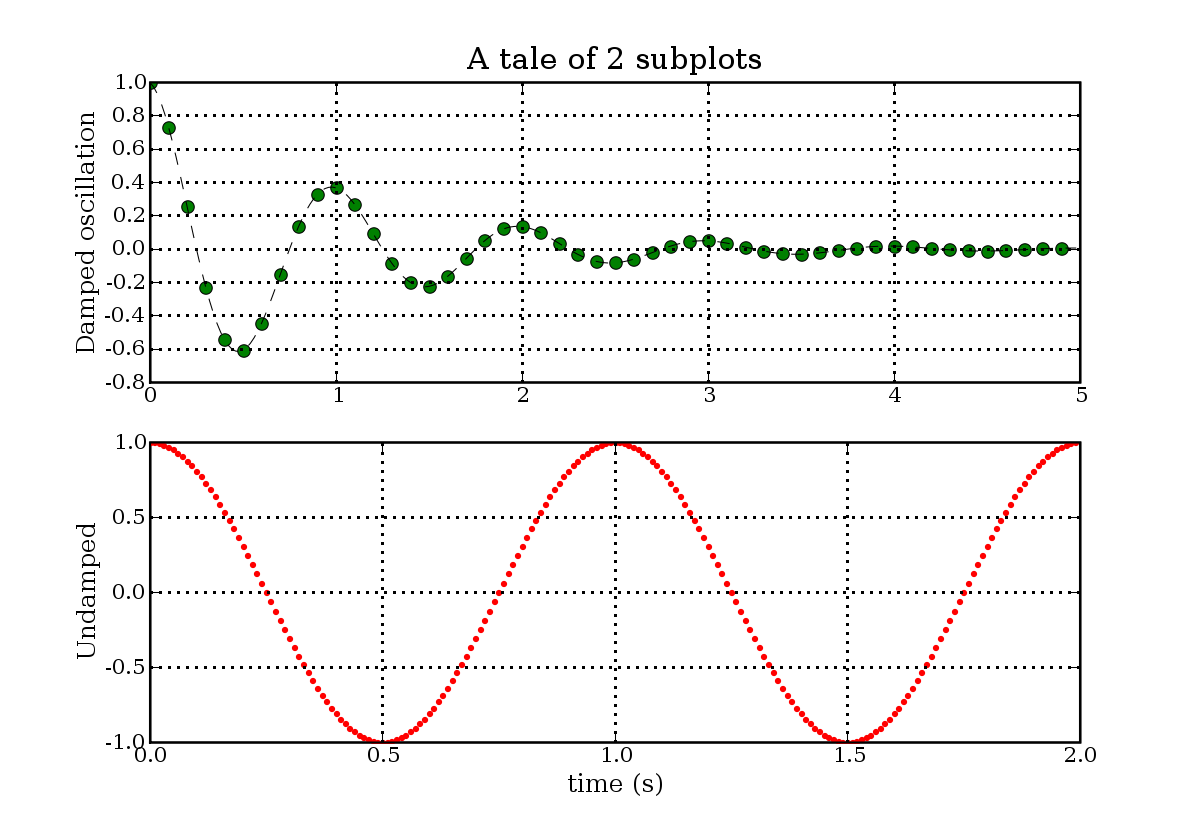
\includegraphics[height=2in, interpolate=true]{data/xyplot}
    \column{0.45\textwidth}
    \begin{block}{Example code}
    \tiny
\begin{lstlisting}
t1 = arange(0.0, 5.0, 0.1)
t2 = arange(0.0, 5.0, 0.02)
t3 = arange(0.0, 2.0, 0.01)
subplot(211)
plot(t1, cos(2*pi*t1)*exp(-t1), 'bo', 
     t2, cos(2*pi*t2)*exp(-t2), 'k')
grid(True)
title('A tale of 2 subplots')
ylabel('Damped')
subplot(212)
plot(t3, cos(2*pi*t3), 'r--')
grid(True)
xlabel('time (s)')
ylabel('Undamped')
\end{lstlisting}
    \end{block}
  \end{columns}
\end{frame}

\begin{frame}[fragile] \frametitle{Errorbar}
  \begin{columns}
    \column{0.5\textwidth}
    \hspace*{-0.5in}
  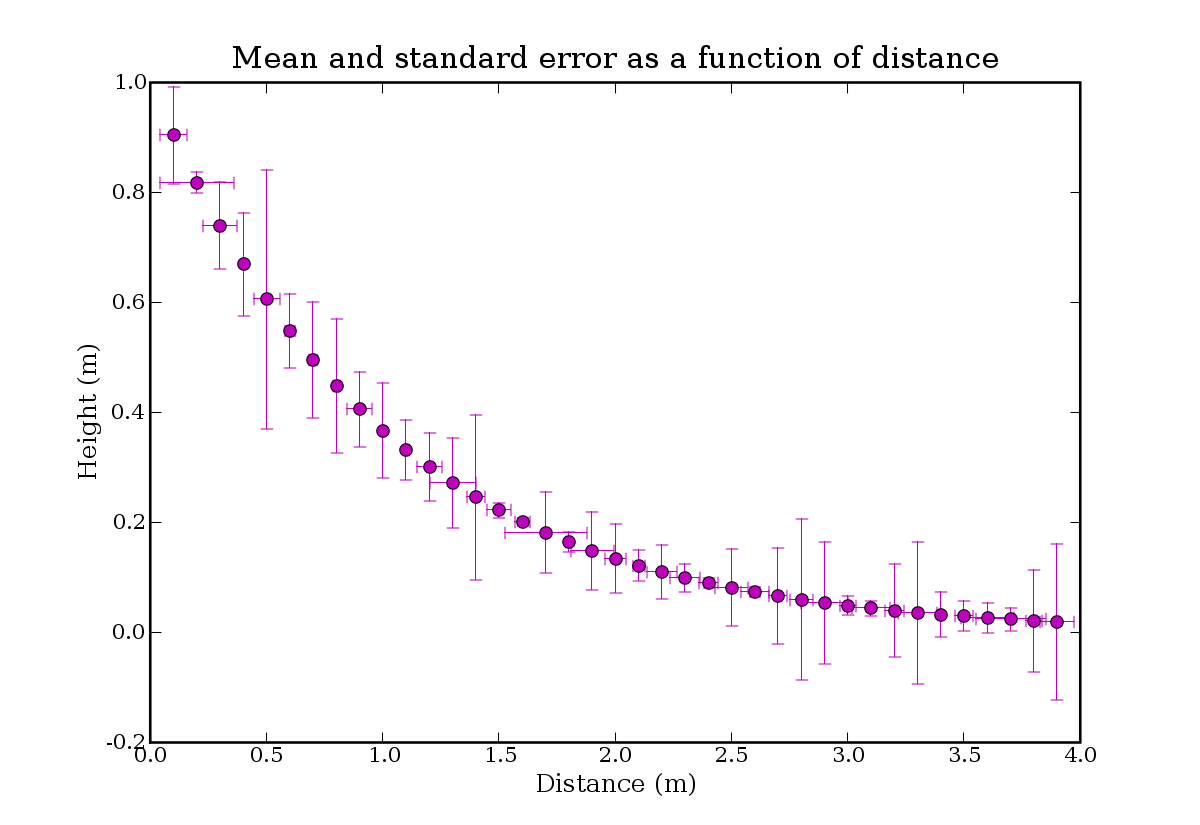
\includegraphics[height=2in, interpolate=true]{data/errorbar}  
    \column{0.45\textwidth}
    \begin{block}{Example code}
    \tiny
\begin{lstlisting}
t = arange(0.1, 4, 0.1)
s = exp(-t)
e = 0.1*abs(randn(len(s)))
f = 0.1*abs(randn(len(s)))
g = 2*e
h = 2*f
errorbar(t, s, [e,g], f, fmt='o')
xlabel('Distance (m)')
ylabel('Height (m)')
title('Mean and standard error '\
      'as a function of distance')
\end{lstlisting}
  \end{block}
\end{columns}
\end{frame}

\begin{frame}[fragile] \frametitle{Semi-log and log-log plots}
  \begin{columns}
    \column{0.5\textwidth}
    \hspace*{-0.5in}
  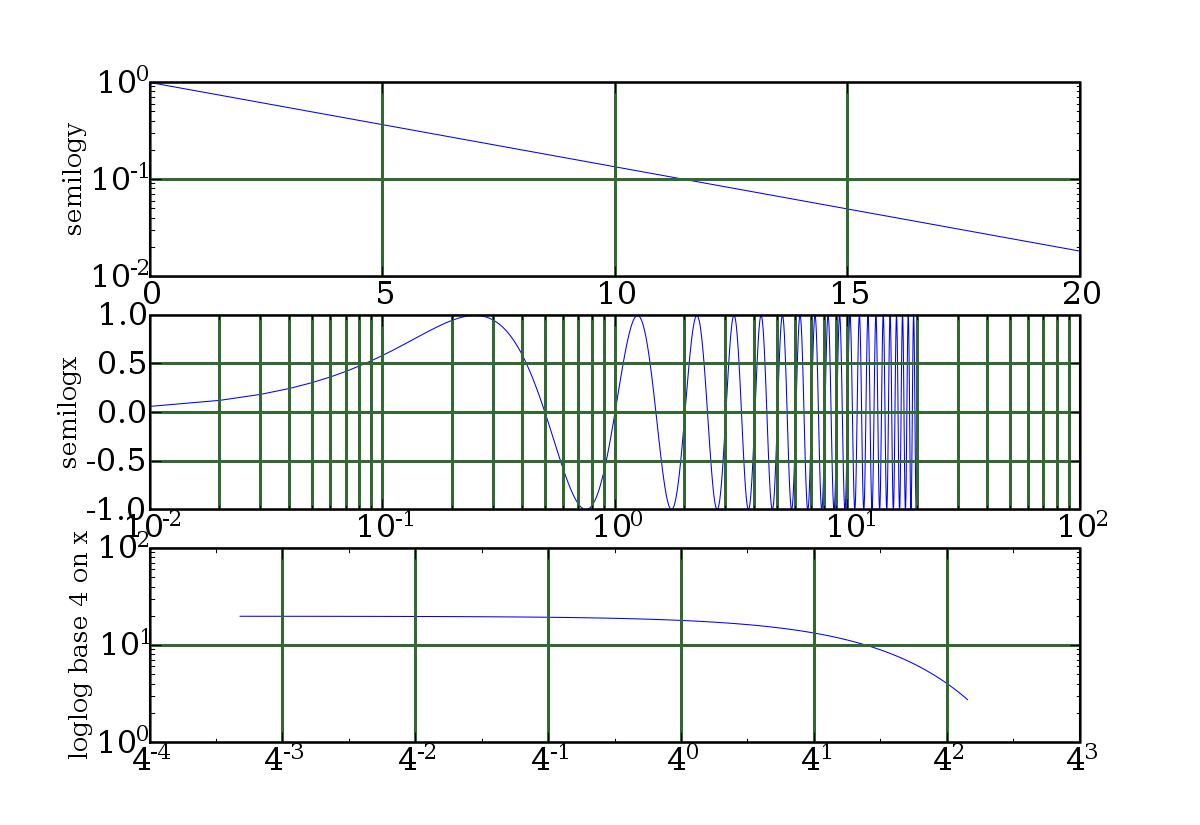
\includegraphics[height=2in, interpolate=true]{data/log}  
    \column{0.45\textwidth}
    \begin{block}{Example code}
    \tiny
\begin{lstlisting}
dt = 0.01
t = arange(dt, 20.0, dt)
subplot(311)
semilogy(t, exp(-t/5.0))
ylabel('semilogy')
grid(True)
subplot(312)
semilogx(t, sin(2*pi*t))
ylabel('semilogx')
grid(True)
# minor grid on too
gca().xaxis.grid(True, which='minor')  
subplot(313)
loglog(t, 20*exp(-t/10.0), basex=4)
grid(True)
ylabel('loglog base 4 on x')
\end{lstlisting}
  \end{block}
\end{columns}
\end{frame}

\begin{frame}[fragile] \frametitle{Histogram}
  \begin{columns}
    \column{0.5\textwidth}
    \hspace*{-0.5in}
  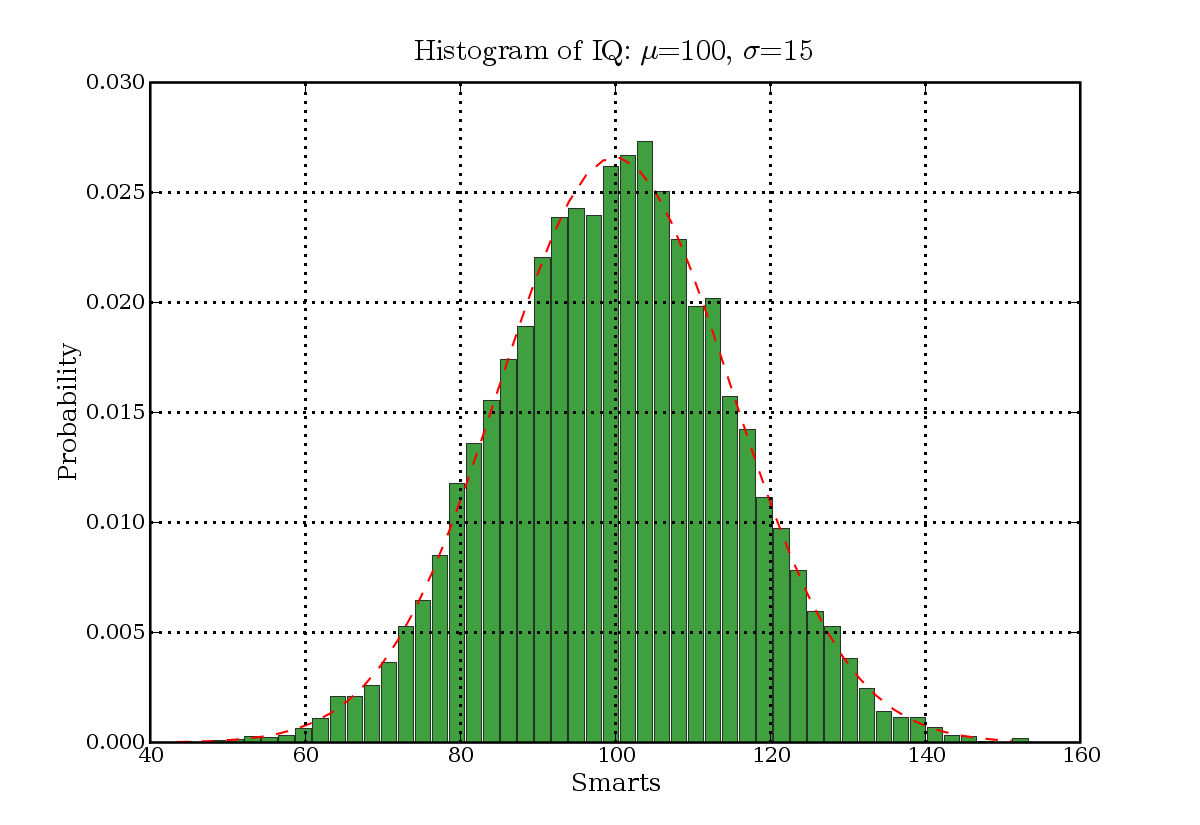
\includegraphics[height=2in, interpolate=true]{data/histogram}  
    \column{0.45\textwidth}
    \begin{block}{Example code}
    \tiny
\begin{lstlisting}
mu, sigma = 100, 15
x = mu + sigma*randn(10000)
# the histogram of the data
n, bins, patches = hist(x, 100, normed=1)
# add a 'best fit' line
y = normpdf( bins, mu, sigma)
l = plot(bins, y, 'r--', linewidth=2)
xlim(40, 160)
xlabel('Smarts')
ylabel('P')
title(r'$\rm{IQ:}\/ \mu=100,\/ \sigma=15$')
\end{lstlisting}
  \end{block}
\end{columns}
\end{frame}

\begin{frame}[fragile] \frametitle{Bar charts}
  \begin{columns}
    \column{0.5\textwidth}
    \hspace*{-0.5in}
  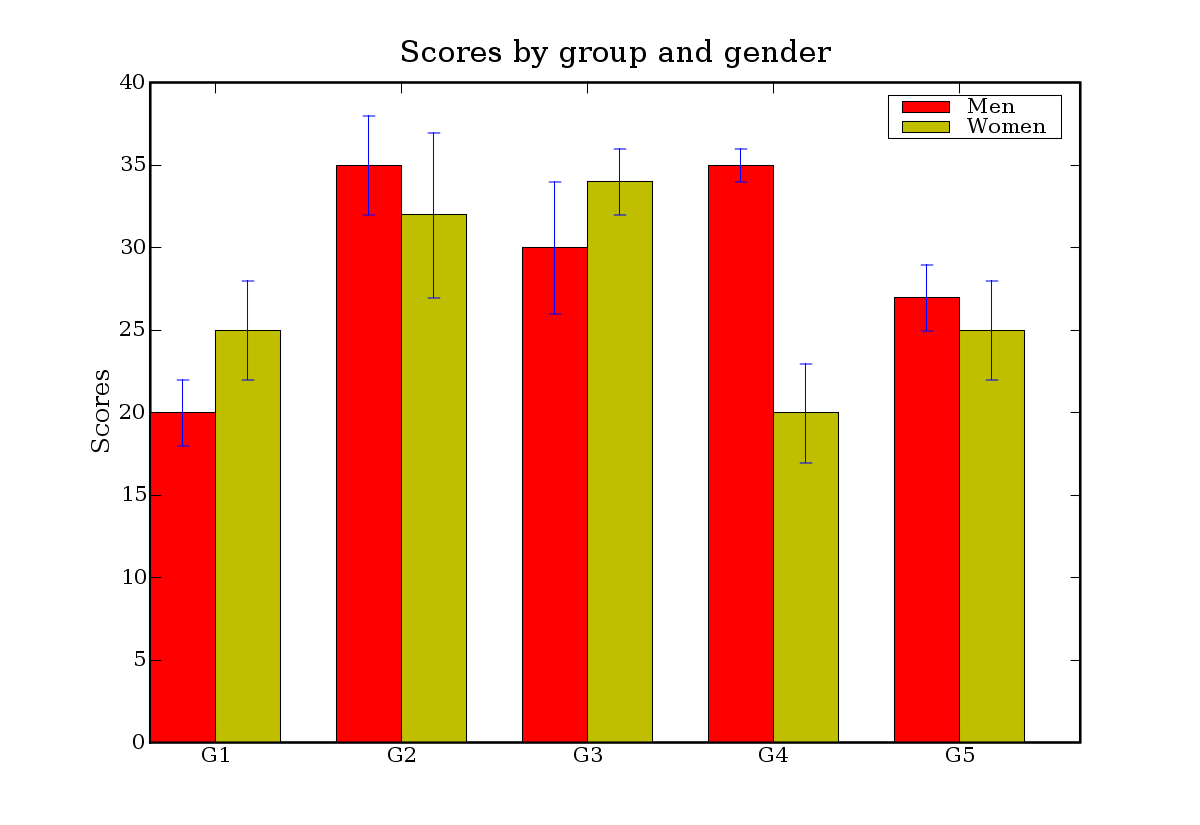
\includegraphics[height=2in, interpolate=true]{data/barchart}  
    \column{0.45\textwidth}
    \begin{block}{Example code}
    \tiny
\begin{lstlisting}
N = 5
menMeans = (20, 35, 30, 35, 27)
menStd =   ( 2,  3,  4,  1,  2)
# the x locations for the groups
ind = arange(N) 
# the width of the bars
width = 0.35       
p1 = bar(ind, menMeans, width, 
         color='r', yerr=menStd)
womenMeans = (25, 32, 34, 20, 25)
womenStd =   ( 3,  5,  2,  3,  3)
p2 = bar(ind+width, womenMeans, width, 
         color='y', yerr=womenStd)
ylabel('Scores')
title('Scores by group and gender')
xticks(ind+width, 
       ('G1', 'G2', 'G3', 'G4', 'G5'))
xlim(-width,len(ind))
yticks(arange(0,41,10))
legend((p1[0], p2[0]), 
       ('Men', 'Women'), shadow=True)
\end{lstlisting}
  \end{block}
\end{columns}
\end{frame}

\begin{frame}[fragile] \frametitle{Pie charts}
  \begin{columns}
    \column{0.5\textwidth}
    \hspace*{-0.4in}
  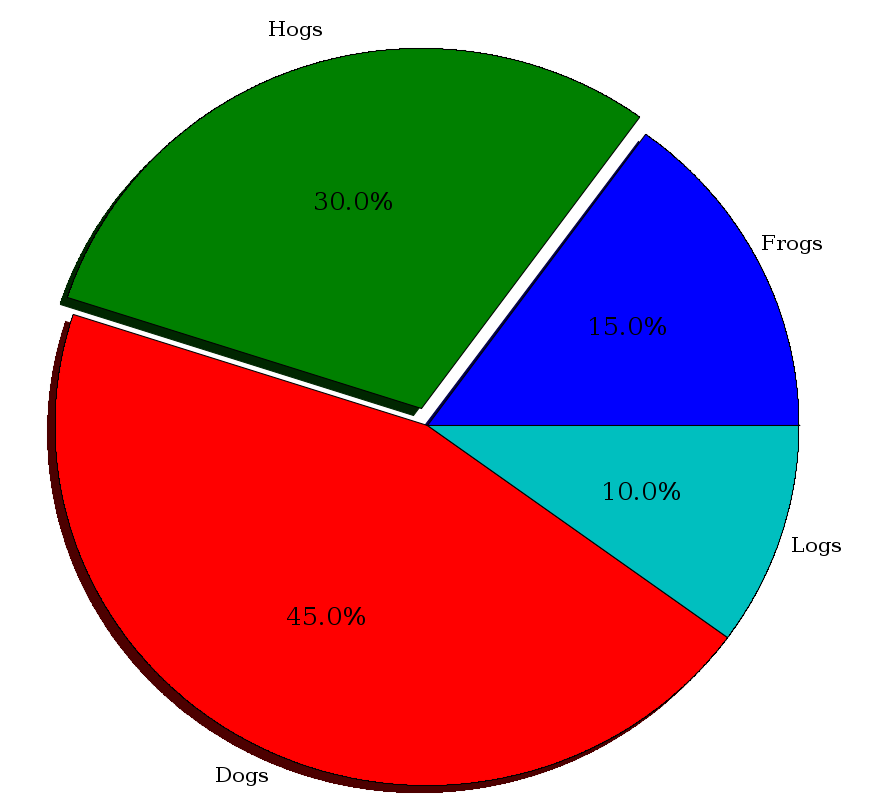
\includegraphics[height=2.0in, interpolate=true]{data/piechart}  
    \column{0.45\textwidth}
    \begin{block}{Example code}
    \tiny
\begin{lstlisting}
# make a square figure and axes
figure(1, figsize=(8,8))
ax = axes([0.1, 0.1, 0.8, 0.8])
labels = 'Frogs', 'Hogs', 'Dogs', 'Logs'
fracs = [15,30,45, 10]
explode=(0, 0.05, 0, 0)
pie(fracs, explode=explode, labels=labels, 
    autopct='%1.1f%%', shadow=True)
title('Raining Hogs and Dogs', 
      bbox={'facecolor':'0.8', 'pad':5})
\end{lstlisting}
  \end{block}
\end{columns}
\end{frame}

\begin{frame}[fragile] \frametitle{Scatter plots}
  \begin{columns}
    \column{0.5\textwidth}
    \hspace*{-0.4in}
  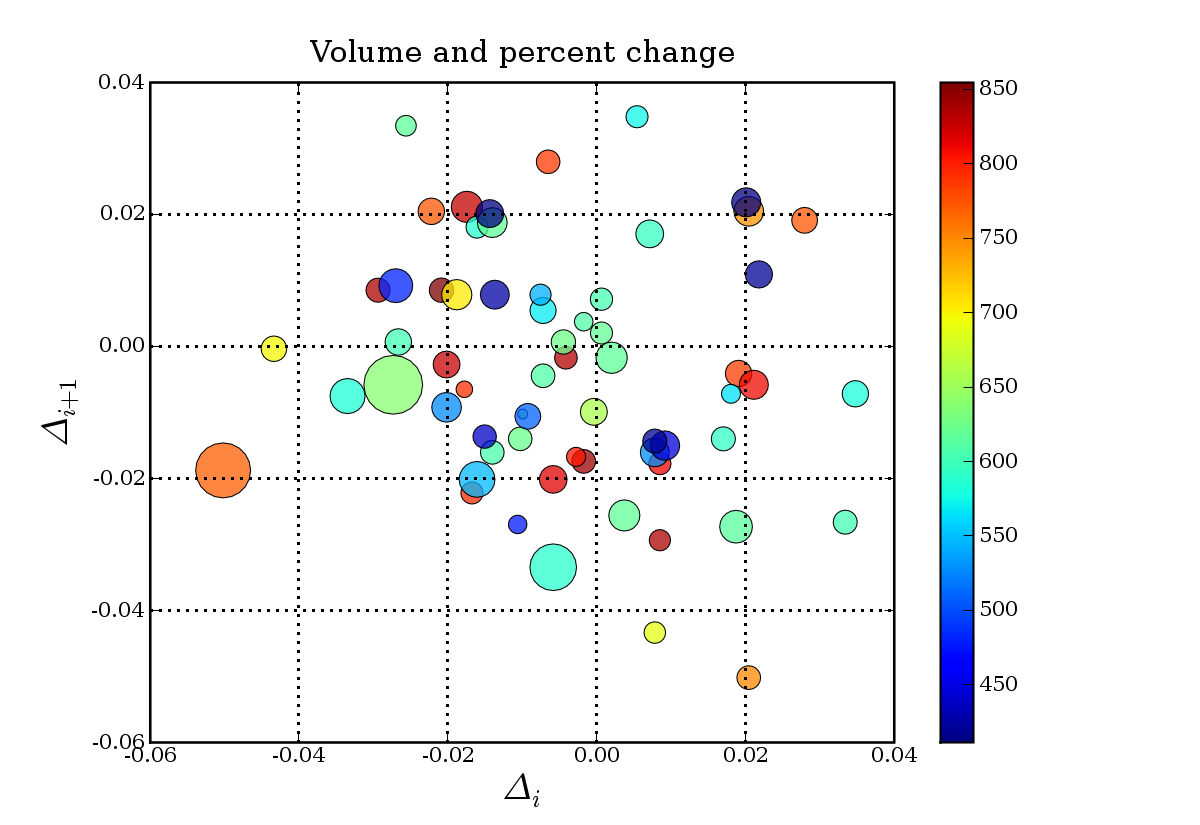
\includegraphics[height=2in, interpolate=true]{data/scatter}  
    \column{0.45\textwidth}
    \begin{block}{Example code}
    \tiny
\begin{lstlisting}
N = 30
x = 0.9*rand(N)
y = 0.9*rand(N)
# 0 to 10 point radiuses
area = pi*(10 * rand(N))**2 
volume = 400 + rand(N)*450
scatter(x,y,s=area, marker='o', c=volume, 
        alpha=0.75)
xlabel(r'$\Delta_i$', size='x-large')
ylabel(r'$\Delta_{i+1}$', size='x-large')
title(r'Volume and percent change')
grid(True)
colorbar()
savefig('scatter')
\end{lstlisting}
  \end{block}
\end{columns}
\end{frame}

\begin{frame}[fragile] \frametitle{Polar}
  \begin{columns}
    \column{0.5\textwidth}
    \hspace*{-0.5in}
  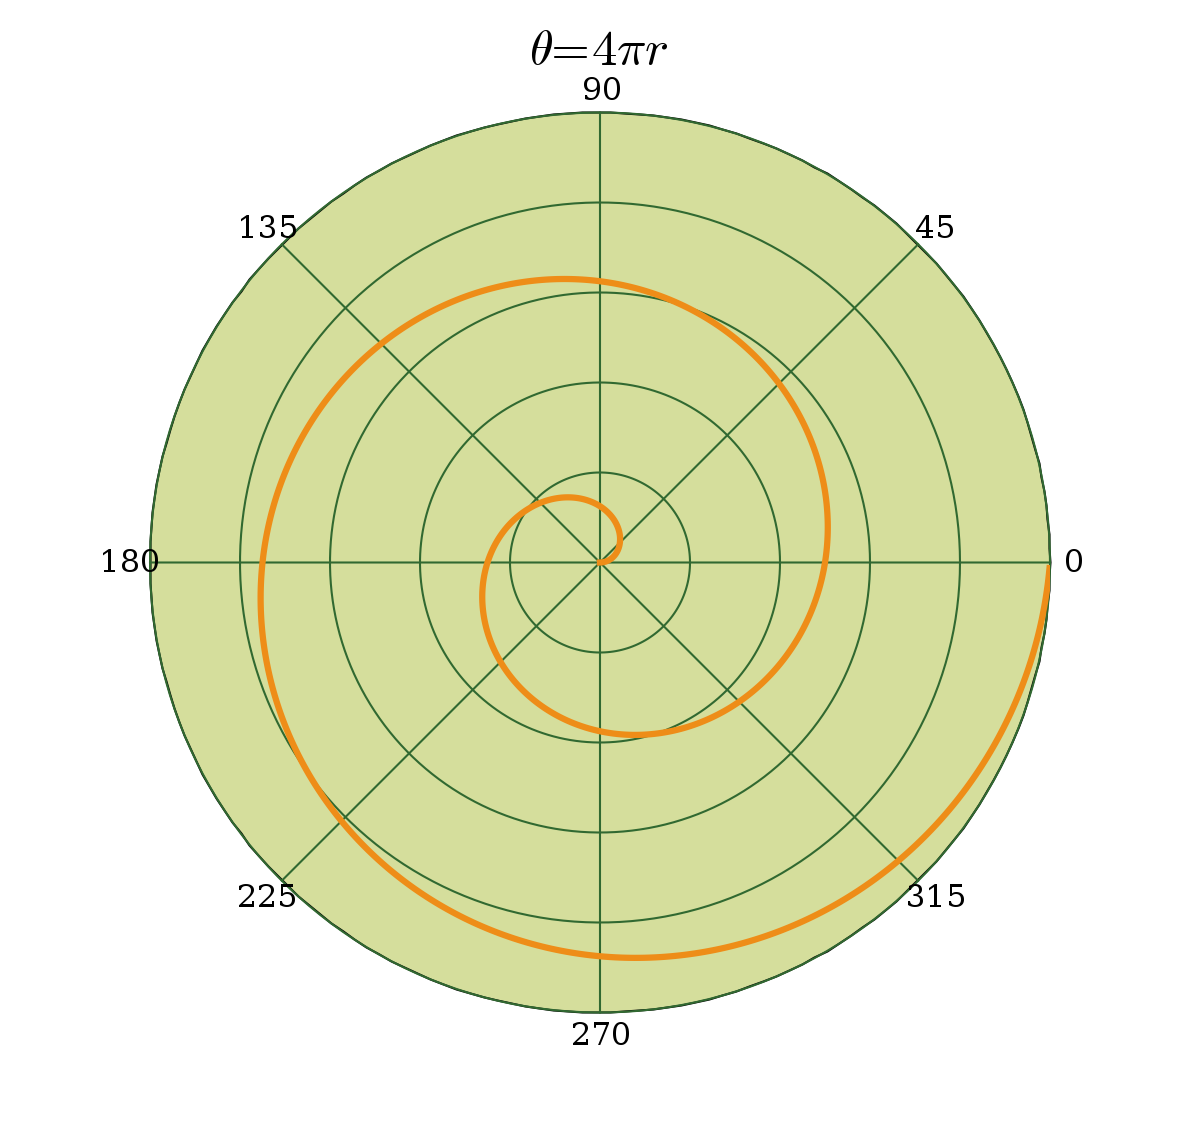
\includegraphics[height=2in, interpolate=true]{data/polar}  
    \column{0.45\textwidth}
    \begin{block}{Example code}
    \tiny
\begin{lstlisting}
figure(figsize=(8,8))
ax = axes([0.1, 0.1, 0.8, 0.8], polar=True, 
          axisbg='#d5de9c')
r = arange(0,1,0.001)
theta = 2*2*pi*r
polar(theta, r, color='#ee8d18', lw=3)
# the radius of the grid labels
setp(ax.thetagridlabels, y=1.075) 
title(r"$\theta=4\pi r", fontsize=20)
\end{lstlisting}
  \end{block}
\end{columns}
\end{frame}

\begin{frame}[fragile] \frametitle{Contours}
  \begin{columns}
    \column{0.45\textwidth}
    \hspace*{-0.5in}
  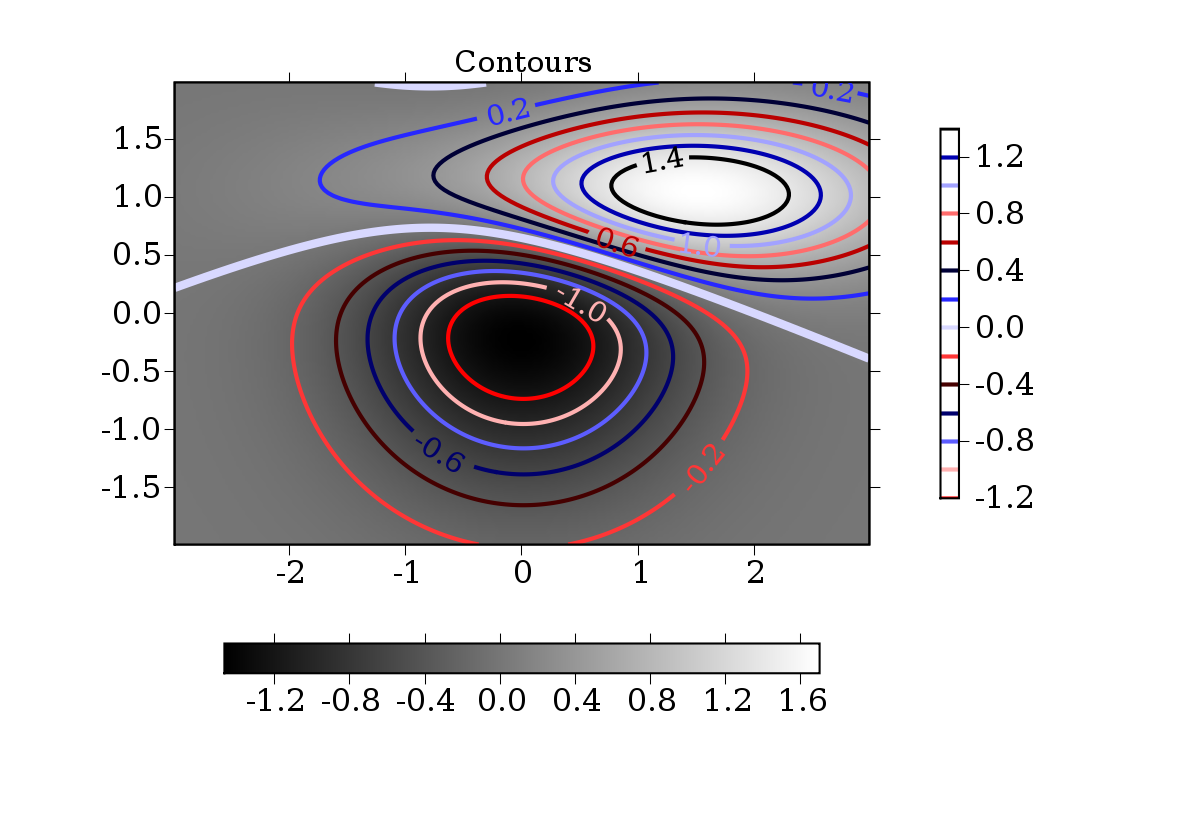
\includegraphics[height=2in, interpolate=true]{data/contour}  
    \column{0.525\textwidth}
    \begin{block}{Example code}
    \tiny
\begin{lstlisting}
x = arange(-3.0, 3.0, 0.025)
y = arange(-2.0, 2.0, 0.025)
X, Y = meshgrid(x, y)
Z1 = bivariate_normal(X, Y, 1.0, 1.0, 0.0, 0.0)
Z2 = bivariate_normal(X, Y, 1.5, 0.5, 1, 1)
# difference of Gaussians
Z = 10.0 * (Z2 - Z1)
im = imshow(Z, interpolation='bilinear', 
            origin='lower',
            cmap=cm.gray, extent=(-3,3,-2,2))
levels = arange(-1.2, 1.6, 0.2)
# label every second level
clabel(CS, levels[1::2],  inline=1,
       fmt='%1.1f', fontsize=14)
CS = contour(Z, levels,
             origin='lower',
             linewidths=2,
             extent=(-3,3,-2,2))
# make a colorbar for the contour lines
CB = colorbar(CS, shrink=0.8, extend='both')
title('Lines with colorbar')
hot(); flag()
\end{lstlisting}
  \end{block}
\end{columns}
\end{frame}

\begin{frame}[fragile] \frametitle{Velocity vectors}
  \begin{columns}
    \column{0.5\textwidth}
    \hspace*{-0.5in}
  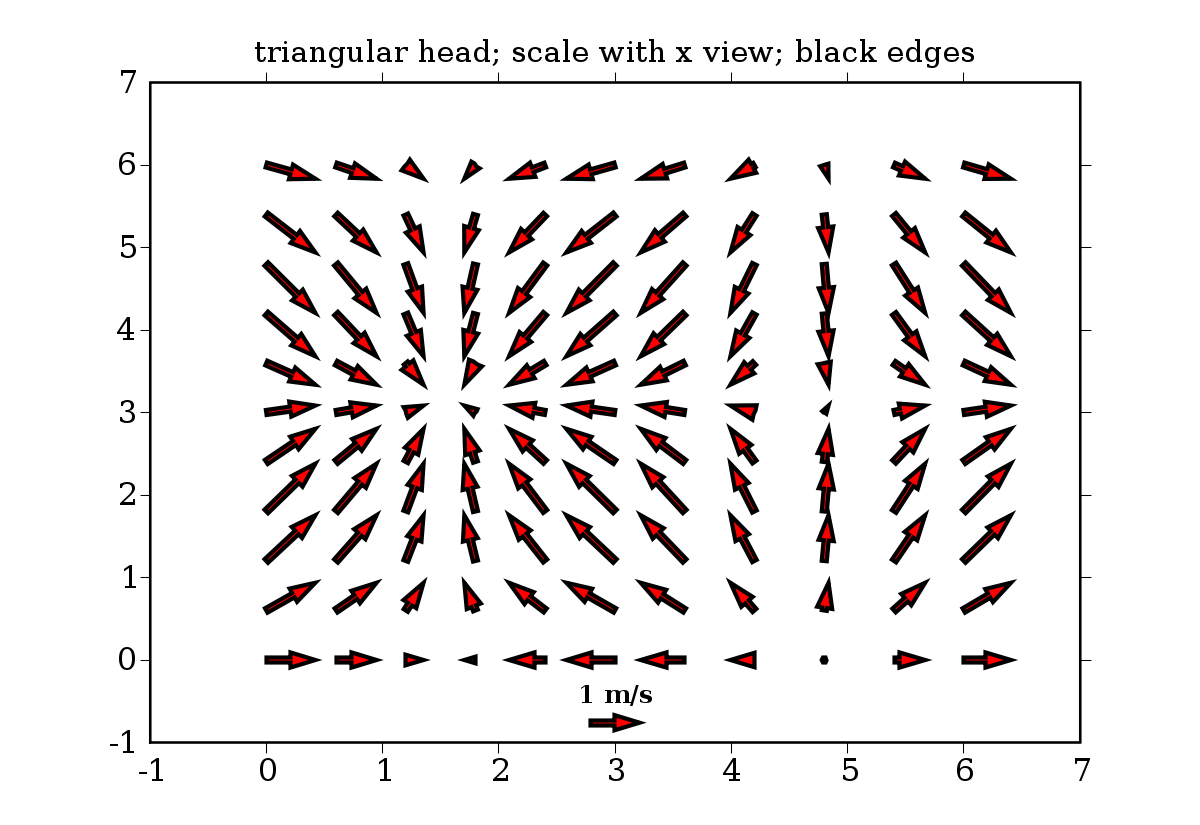
\includegraphics[height=2in, interpolate=true]{data/quiver}  
    \column{0.45\textwidth}
    \begin{block}{Example code}
    \tiny
\begin{lstlisting}
X,Y = meshgrid(arange(0,2*pi,.2),
               arange(0,2*pi,.2) )
U = cos(X)
V = sin(Y)
Q = quiver(X[::3, ::3], Y[::3, ::3], 
           U[::3, ::3], V[::3, ::3],
           color='r', units='x', 
           linewidths=(2,), 
           edgecolors=('k'), 
           headaxislength=5 )
qk = quiverkey(Q, 0.5, 0.03, 1, '1 m/s', 
               fontproperties=
               {'weight': 'bold'})
axis([-1, 7, -1, 7])
title('triangular head; scale '\
      'with x view; black edges')
\end{lstlisting}
  \end{block}
\end{columns}
\end{frame}

\begin{frame}[fragile] \frametitle{Maps}
  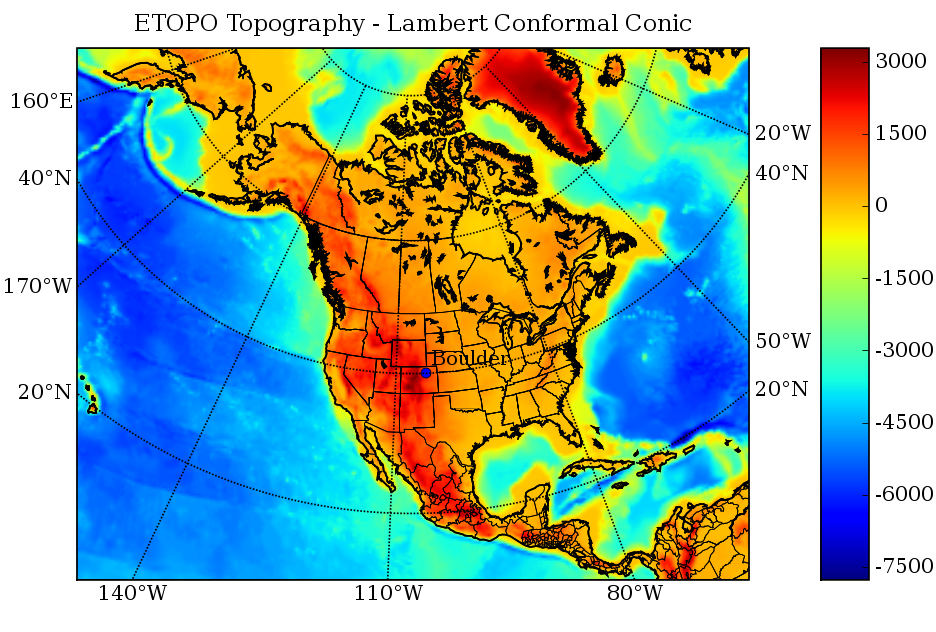
\includegraphics[height=2.5in, interpolate=true]{data/plotmap}  
  \begin{center}
    \tiny
    For details see \url{http://matplotlib.sourceforge.net/screenshots/plotmap.py}
  \end{center}
\end{frame}


\subsection{SciPy}

\begin{frame}
  \frametitle{Using \texttt{SciPy}}
  \begin{itemize}
  \item SciPy is Open Source software for mathematics, science, and
    engineering
  \item \typ{import scipy}
  \item Built on NumPy
  \item Provides modules for statistics, optimization, integration,
    linear algebra, Fourier transforms, signal and image processing,
    genetic algorithms, ODE solvers, special functions, and more
  \item Used widely by scientists world over
  \item Details are beyond the scope of this tutorial
  \end{itemize}
\end{frame}

\section{Standard library}

\subsection{Quick Tour}

\begin{frame}
  \frametitle{Standard library}
  \begin{itemize}
  \item Very powerful
  \item ``Batteries included''
  \item Example standard modules taken from the tutorial
    \begin{itemize}
    \item Operating system interface: \typ{os}
    \item System, Command line arguments: \typ{sys}
    \item Regular expressions: \typ{re}
    \item Math: \typ{math}, \typ{random}
    \item Internet access: \typ{urllib2}, \typ{smtplib}
    \item Data compression: \typ{zlib}, \typ{gzip}, \typ{bz2},
      \typ{zipfile}, and \typ{tarfile}
    \item Unit testing: \typ{doctest} and \typ{unittest}
    \item And a whole lot more!
    \end{itemize}
  \item Check out the Python Library reference:
    \url{http://docs.python.org/lib/lib.html}
  \end{itemize}
\end{frame}

\begin{frame}[fragile]
  \frametitle{Stdlib: examples}
\begin{lstlisting}
>>> import os
>>> os.system('date')
Fri Jun 10 22:13:09 IST 2005
0
>>> os.getcwd()
'/home/prabhu'
>>> os.chdir('/tmp')
>>> import os
>>> dir(os)
<returns a list of all module functions>
>>> help(os)
<extensive manual page from module's docstrings>
\end{lstlisting}
\end{frame}

\begin{frame}[fragile]
  \frametitle{Stdlib: examples}
\begin{lstlisting}
>>> import sys
>>> # Print the list of command line args to Python
... print sys.argv 
['']
>>> import re # Regular expressions
>>> re.findall(r'\bf[a-z]*', 
... 'which foot or hand fell fastest')
['foot', 'fell', 'fastest']
>>> re.sub(r'(\b[a-z]+) \1', r'\1', 
... 'cat in the the hat')
'cat in the hat'
\end{lstlisting}
\end{frame}

\begin{frame}[fragile]
  \frametitle{Stdlib: examples}
\begin{lstlisting}
>>> import math
>>> math.cos(math.pi / 4.0)
0.70710678118654757
>>> math.log(1024, 2)
10.0
>>> import random
>>> random.choice(['apple', 'pear', 'banana'])
'pear'
\end{lstlisting}
\end{frame}

\begin{frame}[fragile]
  \frametitle{Stdlib: examples}
\begin{lstlisting}
>>> import urllib2
>>> f = urllib2.urlopen('http://www.python.org/')
>>> print f.read(100)
<!DOCTYPE html PUBLIC "-//W3C//DTD HTML 4.01 Transitional//EN">
<?xml-stylesheet href="./css/ht2html
\end{lstlisting}
\end{frame}

\begin{frame}[fragile]
  \frametitle{Stdlib: examples}
\begin{lstlisting}
>>> import zlib
>>> s = 'witch which has which witches wrist watch'
>>> len(s)
41
>>> t = zlib.compress(s)
>>> len(t)
37
>>> zlib.decompress(t)
'witch which has which witches wrist watch'
>>> zlib.crc32(t)
-1438085031
\end{lstlisting}
\end{frame}

\begin{frame}
  \frametitle{Summary}
  \begin{itemize}
  \item Introduced Python
  \item Basic syntax
  \item Basic types and data structures
  \item Control flow
  \item Functions
  \item Modules
  \item Exceptions
  \item Classes
  \item Standard library
  \end{itemize}
\end{frame}

\end{document}

\subsection{Basic data structures}
\begin{frame}{Lists}
  \begin{itemize}
    \item \texttt{species = [ 'humans', 'orcs', 'elves', 'dwarves' ]}
    \item \texttt{ ids = [ 107, 109, 124, 141, 142, 144 ]}
    \item \texttt{ oneliners = [ 'I will be back', 'Do or do not! No try!!', 42 ] }
  \end{itemize}

  \begin{block}{List operations}
    ids + [ 100, 102 ]\\
    species.append( 'unicorns')\\
    print oneliners[ 1 ]\\
    look up \alert{docs.python.org/tutorial/datastructures.html}
  \end{block}
\end{frame}
\end{document}
\section{Python Tutorial}
\subsection{Preliminaries}
\begin{frame}
  \frametitle{Using the interpreter}
  \begin{itemize}
  \item Starting up: \typ{python} or \typ{ipython}
  \item Quitting: \typ{Control-D} or \typ{Control-Z} (on Win32)
  \item Can use it like a calculator
  \item Can execute one-liners via the \typ{-c} option:
    \typ{python -c "print 'hello world'"}
  \item Other options via \typ{python -h}
  \end{itemize}
\end{frame}

\begin{frame}
  \frametitle{IPython}
  \begin{itemize}
  \item Recommended interpreter, IPython:
    \url{http://ipython.scipy.org}
  \item Better than the default Python shell
  \item Supports tab completion by default
  \item Easier object introspection
  \item Shell access!
  \item Command system to allow extending its own behavior
  \item Supports history (across sessions) and logging
  \item Can be embedded in your own Python code
  \item Support for macros
  \item A flexible framework for your own custom interpreter
  \item Other miscellaneous conveniences
  \item We'll get back to this later
  \end{itemize}
\end{frame}

\begin{frame}[fragile]
  \frametitle{Basic IPython features}
  \begin{itemize}
  \item Startup: \verb+ipython [options] files+
    \begin{itemize}
    \item \verb+ipython [-wthread|-gthread|-qthread]+:
      Threading modes to support wxPython, pyGTK and Qt
    \item \verb+ipython -pylab+: Support for matplotlib
    \end{itemize}
  \item TAB completion:
    \begin{itemize}
    \item Type \verb+object_name.<TAB>+ to see list of options
    \item Also completes on file and directory names
    \end{itemize}
  \item \verb+object?+ shows docstring/help for any Python object
  \item \verb+object??+ presents more docs (and source if possible)
  \item Debugging with \verb+%pdb+ magic: pops up pdb on errors
  \item Access history (saved over earlier sessions also)
    \begin{itemize}
    \item Use \texttt{<UpArrow>}: move up history
    \item Use \texttt{<Ctrl-r> string}: search history backwards
    \item Use \texttt{Esc >}: get back to end of history
    \end{itemize}
  \item \verb+%run [options] file[.py]+ lets you run Python code
  \end{itemize}
\end{frame}
% LocalWords:  BDFL Guido Rossum PSF Nokia OO Zope CMS RedHat SciPy MayaVi spam
% LocalWords:  IPython ipython stdin TypeError dict int elif PYTHONPATH IOError
% LocalWords:  namespace Namespaces SyntaxError ZeroDivisionError NameError str
% LocalWords:  ValueError subclassed def


  \item Types are of two kinds: \alert{mutable} and \alert{immutable}
  \item Immutable types: numbers, strings, \typ{None} and tuples
  \item Immutables cannot be changed ``in-place''
  \item Mutable types: lists, dictionaries, instances, etc.
  \item Mutable objects can be ``changed''
  \end{itemize}


\begin{frame}
  \frametitle{Important!}
  \begin{itemize}
    \item Assignment to an object is by reference
    \item Essentially, \alert{names are bound to objects}
  \end{itemize}
\end{frame}


\end{document}
\begin{frame}[fragile]
  \frametitle{Dictionaries}
  \begin{itemize}
  \item Associative arrays/mappings
  \item Indexed by ``keys'' (keys must be immutable)
  \item \typ{dict[key] = value}
  \item \typ{keys()} returns all keys of the dict
  \item \typ{values()} returns the values of the dict
  \item \verb+has_key(key)+ returns if \typ{key} is in the dict
  \end{itemize}
\end{frame}

\begin{frame}[fragile]
  \frametitle{Dictionaries: example}
  \begin{lstlisting}
>>> tel = {'jack': 4098, 'sape': 4139}
>>> tel['guido'] = 4127
>>> tel
{'sape': 4139, 'guido': 4127, 'jack': 4098}
>>> tel['jack']
4098
>>> del tel['sape']
>>> tel['irv'] = 4127
>>> tel
{'guido': 4127, 'irv': 4127, 'jack': 4098}
>>> tel.keys()
['guido', 'irv', 'jack']
>>> tel.has_key('guido')
True
  \end{lstlisting}
\end{frame}

\subsection{Control flow, functions}



\begin{frame}[fragile]
  \frametitle{\typ{If} example}
  \begin{lstlisting}
>>> a = ['cat', 'window', 'defenestrate']
>>> if 'cat' in a:
...    print "meaw"
...
meaw
>>> pets = {'cat': 1, 'dog':2, 'croc': 10}
>>> if 'croc' in pets:
...    print pets['croc']
...
10
  \end{lstlisting}
\end{frame}

\begin{frame}[fragile]
  \frametitle{\typ{for} example}
  \begin{lstlisting}
>>> a = ['cat', 'window', 'defenestrate']
>>> for x in a:
...     print x, len(x)
...
cat 3
window 6
defenestrate 12
>>> knights = {'gallahad': 'the pure', 
... 'robin': 'the brave'}
>>> for k, v in knights.iteritems():
...     print k, v
...
gallahad the pure
robin the brave
\end{lstlisting}
\end{frame}
